\documentclass[aspectratio=169]{beamer}
\usetheme{metropolis}
\usepackage{metropolis-upm}

\usepackage[utf8]{inputenc}
\usepackage[T1]{fontenc}
\usepackage[spanish,english]{babel}
\usepackage{booktabs}
\usepackage{graphicx}
\usepackage{array}

\metroset{sectionpage=none}

\title{Vulnerability Analysis of Port Infrastructure\\Using Satellite InSAR and Probabilistic Methods}
\subtitle{De mediciones satelitales a evidencia para decision en puertos}
\author{Jaime Sanchez Fernandez}
\date{Defensa de tesis doctoral}
\institute{Universidad Politecnica de Madrid}
\titlegraphic{\hfill\includegraphics[height=2.2cm]{upm-logo.png}}

\begin{document}

\maketitle

\begin{frame}{Guion de la presentacion}
  \tableofcontents
\end{frame}

\section{Introduccion}

\begin{frame}{Motivacion}
  \begin{itemize}
    \item Los puertos son infraestructuras criticas para transporte, energia e industria.
    \item Su estado geometrico condiciona operatividad, mantenimiento y riesgo.
    \item La monitorizacion debe ser periodica, comparable y trazable.
  \end{itemize}
\end{frame}

\begin{frame}{Complejidad del activo portuario}
  \begin{itemize}
    \item Un puerto no es una estructura unica: diques, muelles, rellenos, terminales y tanques.
    \item Coexisten tipologias estructurales, contextos geotecnicos y exposiciones muy distintas.
    \item Una lectura unica de la deformacion no es suficiente.
  \end{itemize}
\end{frame}

\begin{frame}{Limites de la auscultacion tradicional}
  \begin{itemize}
    \item Nivelacion, GNSS, topografia y LiDAR aportan gran precision.
    \item Pero suelen ser locales, costosos y dependientes de campanas puntuales.
    \item Falta una capa amplia y recurrente de observacion a escala portuaria.
    \item InSAR aporta cobertura, recurrencia y archivo historico como complemento.
  \end{itemize}
\end{frame}

\begin{frame}{Tres ambiguedades}
  \begin{enumerate}
    \item Ambiguedad de senal.
    \item Ambiguedad espacial.
    \item Ambiguedad interpretativa.
  \end{enumerate}
  \vspace{0.4cm}
  Detectar movimiento no equivale a emitir un diagnostico: la tesis se estructura para resolver estas tres ambiguedades como una unica cadena metodologica.
\end{frame}

\begin{frame}{Marco de riesgo}
  \begin{itemize}
    \item En el sistema portuario, el riesgo puede expresarse como $R = [P, V, C]$.
    \item $P$: presencia de cambio; $V$: vulnerabilidad geometrica; $C$: consecuencia.
    \item La tesis aporta evidencia observacional para $P$ y $V$, y organiza la base espacial para $C$.
  \end{itemize}
\end{frame}

\begin{frame}{VAI y pipeline de la tesis}
  \begin{itemize}
    \item El \textbf{VAI} es la unidad de observacion: coherencia estructural, funcional y geotecnica.
    \item La tesis sigue un pipeline: \textbf{medida $\rightarrow$ atribucion $\rightarrow$ interpretacion}.
    \item Objetivo final: convertir cinematica satelital en evidencia util para decision.
  \end{itemize}
\end{frame}

\section{Capitulo 2: Medida}

\begin{frame}{Capitulo 2: el problema de medida}
  \begin{itemize}
    \item El entorno portuario dificulta la observacion interferometrica.
    \item Antes de interpretar deformacion, hay que construir una capa cinematica util.
    \item El objetivo del capitulo es mejorar densidad, cobertura y reproducibilidad.
  \end{itemize}
\end{frame}

\begin{frame}{Retos de senal en puertos}
  \begin{itemize}
    \item Interfaz tierra-mar, escolleras y superficies mixtas.
    \item Mezcla de dispersores persistentes y distribuidos.
    \item Perdidas de coherencia en zonas de alto interes ingenieril.
  \end{itemize}
\end{frame}

\begin{frame}{Por que trabajar con CSLC}
  \begin{itemize}
    \item Los productos \texttt{L2-CSLC} ofrecen una base coregistrada y geocodificada.
    \item Reducen barreras de entrada respecto a flujos legados desde \texttt{L1-SLC}.
    \item Facilitan trazabilidad e integracion posterior con GIS y otras fuentes.
  \end{itemize}
\end{frame}

\begin{frame}{Flujo general del capitulo 2}
  \begin{itemize}
    \item Ingestion de productos CSLC con \texttt{COMPASS} e \texttt{ISCE3}.
    \item \texttt{Phase linking} con \texttt{MiaPLpy}.
    \item Desempaquetado, red interferometrica e inversion temporal.
  \end{itemize}
\end{frame}

\begin{frame}{Correcciones y phase linking}
  \begin{itemize}
    \item Correcciones tipo \texttt{MAGIC}/ETAD para Doppler, azimut y efectos geometricos.
    \item Modelado de troposfera, ionosfera y mareas terrestres.
    \item Mejora de consistencia geolocalizada en la pila temporal.
    \item \texttt{Phase linking}: mas cobertura util en zonas dominadas por dispersores distribuidos.
  \end{itemize}
\end{frame}

\begin{frame}{Red interferometrica e inversion}
  \begin{itemize}
    \item \texttt{SNAPHU} para el desempaquetado.
    \item Red redundante para evitar desconexiones y mejorar estabilidad.
    \item Inversion robusta ponderada por coherencia temporal.
  \end{itemize}
\end{frame}

\begin{frame}{Coherencia y tipo de dispersor}
  \centering
  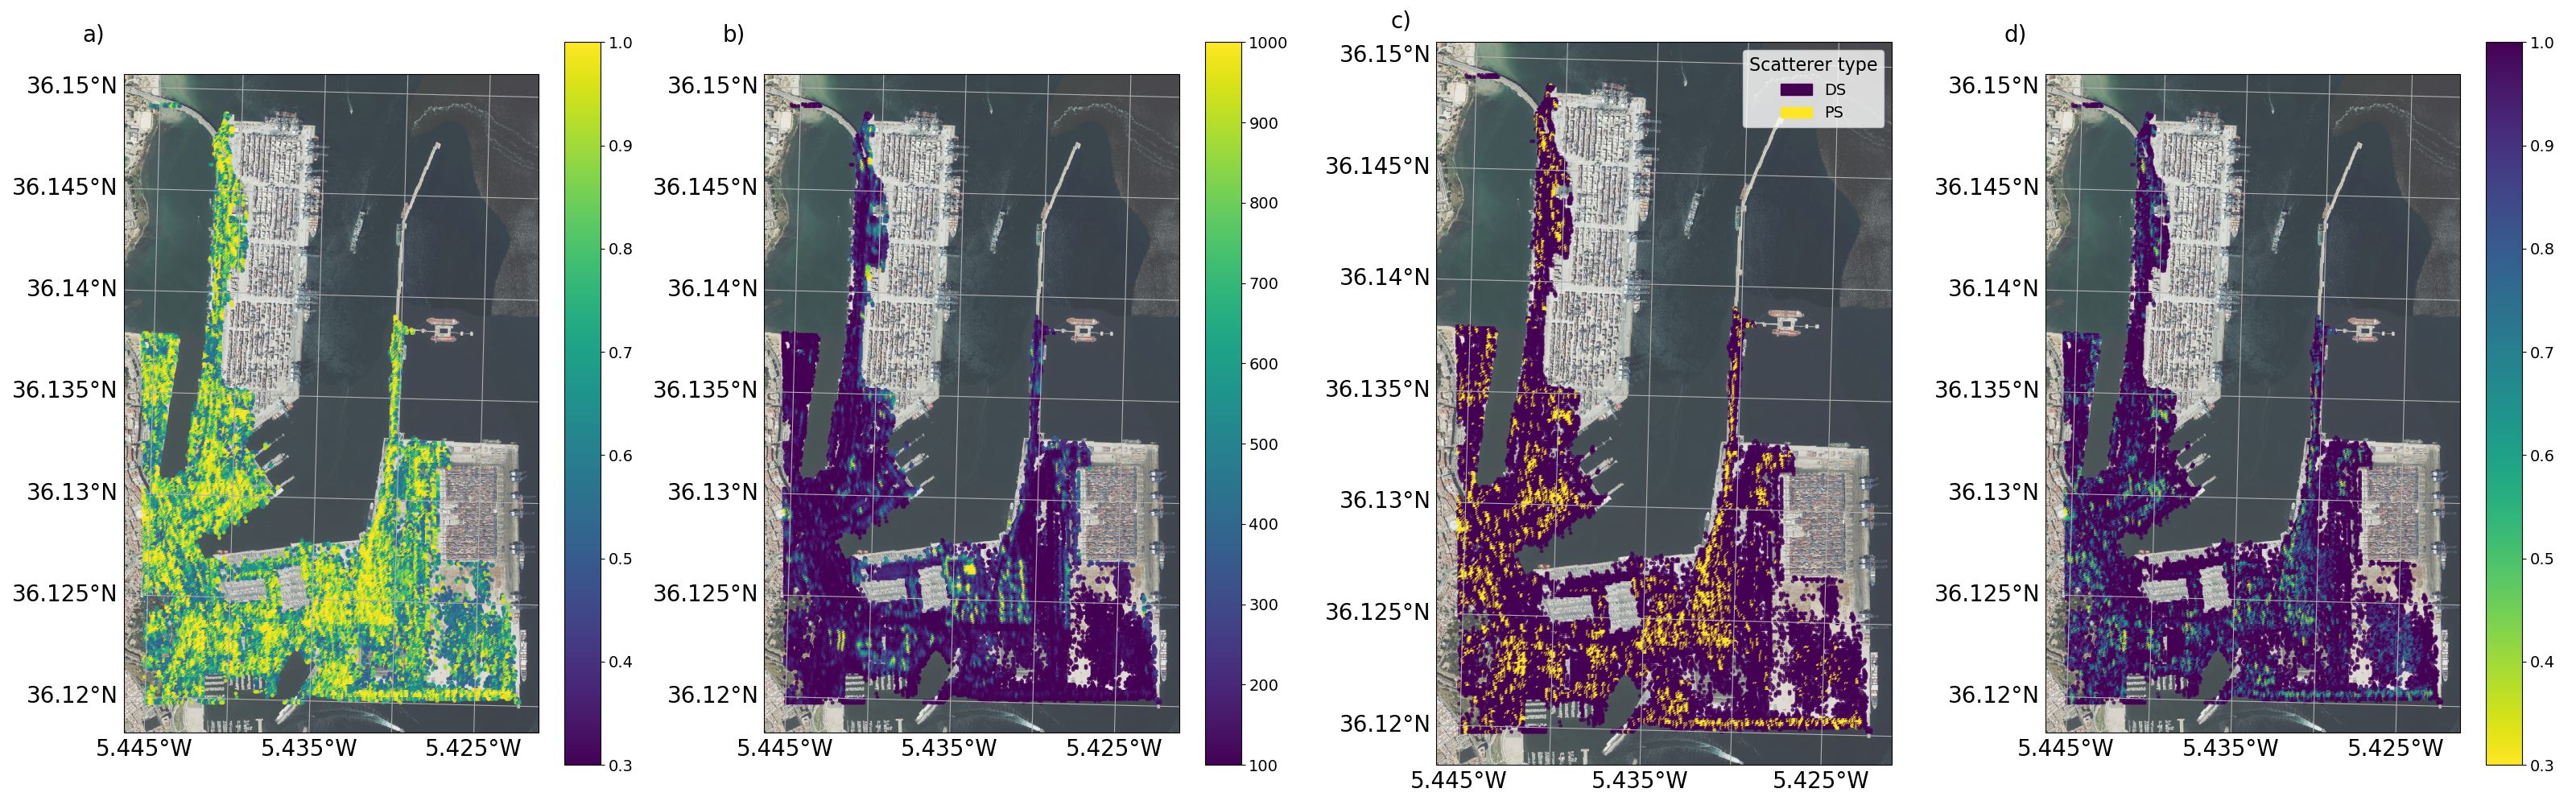
\includegraphics[width=0.95\linewidth]{figures/ch2_coherence_amplitude.png}
\end{frame}

\begin{frame}{Resultado principal: cobertura y densidad}
  \centering
  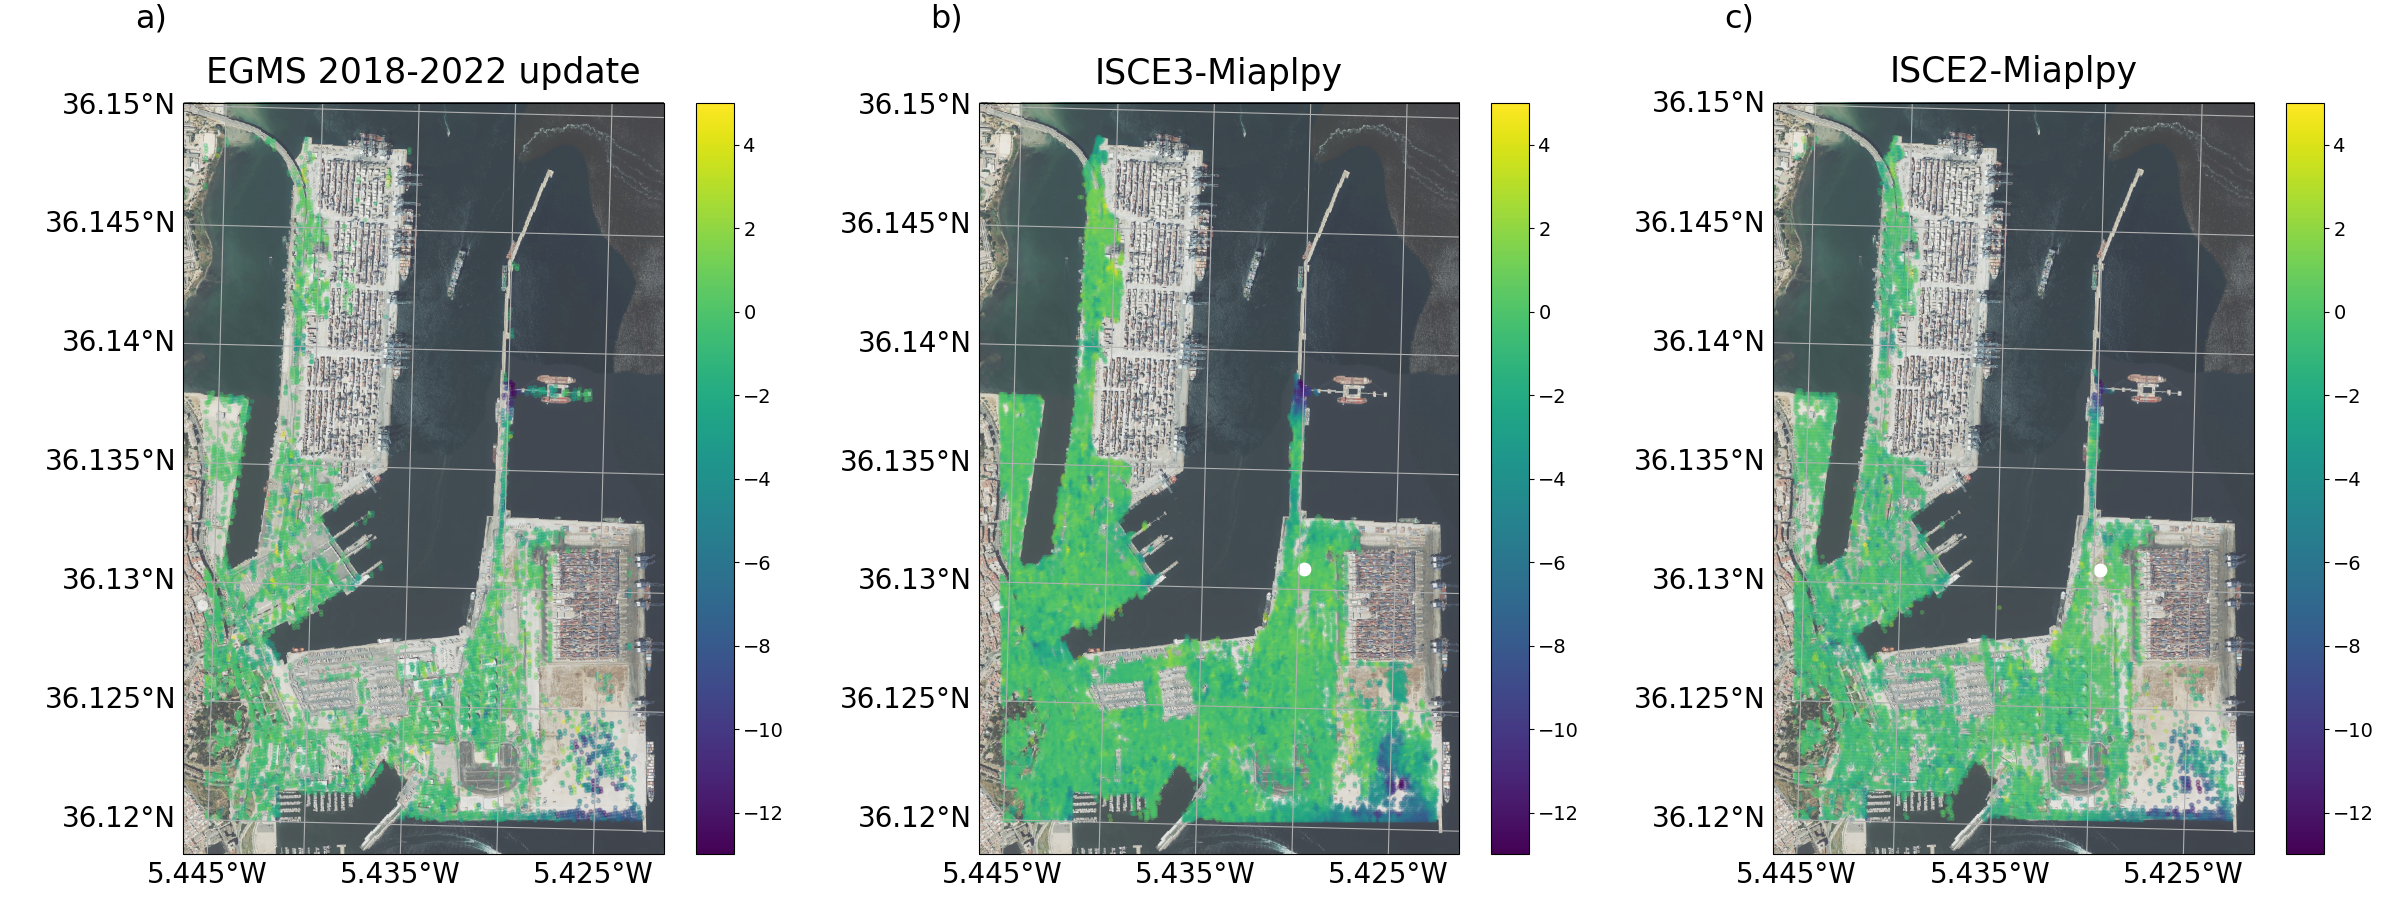
\includegraphics[width=0.98\linewidth]{figures/ch2_velocity_comparison.png}
\end{frame}

\begin{frame}{Resultado principal: comparativa estadistica}
  \centering
  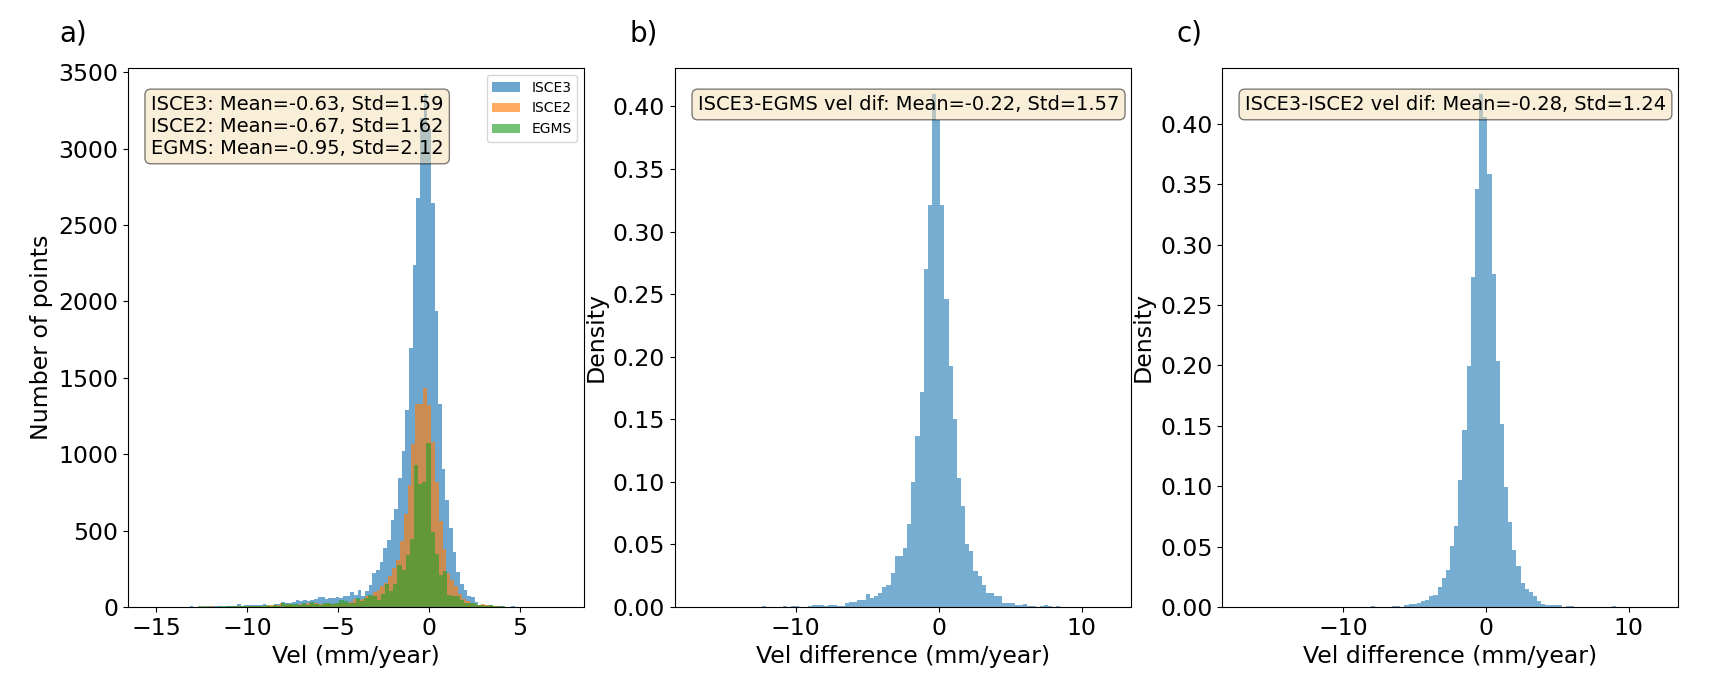
\includegraphics[width=0.92\linewidth]{figures/ch2_velocity_histograms.png}
\end{frame}

\begin{frame}{Resultado principal: validacion con series temporales}
  \centering
  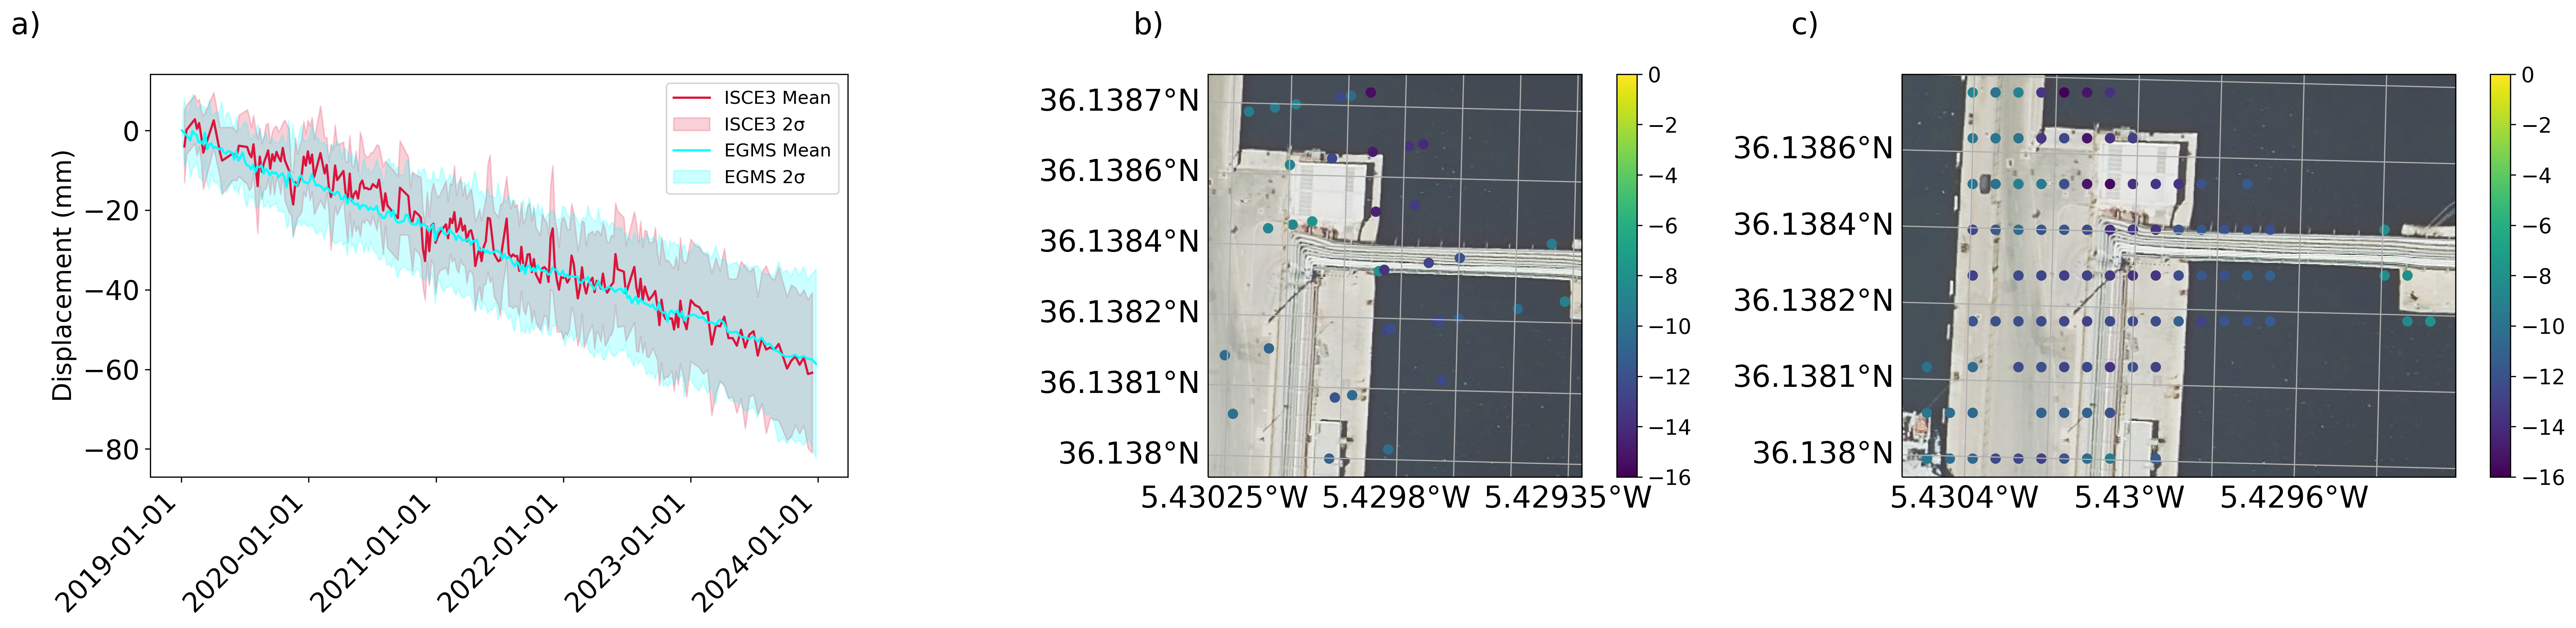
\includegraphics[width=0.95\linewidth]{figures/ch2_ts_evos.png}
\end{frame}

\begin{frame}{Mensaje del capitulo 2}
  \begin{itemize}
    \item El aporte no es solo procesar de otra forma.
    \item El aporte es construir una base observacional mas densa, trazable y util.
    \item Esta capa de medida es la base de los capitulos posteriores.
  \end{itemize}
\end{frame}

\section{Capitulo 3: Atribucion}

\begin{frame}{Capitulo 3: el problema de atribucion}
  \begin{itemize}
    \item Una nube de puntos InSAR sigue siendo insuficiente si no sabemos a que activo pertenece.
    \item En puertos, la geometria radar introduce \texttt{shadow}, \texttt{layover} e incertidumbre transversal.
    \item El objetivo es anclar la cinematica a la geometria real del activo.
  \end{itemize}
\end{frame}

\begin{frame}{Factores criticos y rol del LiDAR}
  \begin{itemize}
    \item Geometrias verticales y complejas: tanques, muros, gruas, estructuras metalicas.
    \item Dinamica operativa y ambiental: traficos, apilamientos, atmosfera marina.
    \item La calidad observacional depende de coherencia y compatibilidad geometrica.
    \item InSAR observa el tiempo; LiDAR describe la geometria 3D y mejora la atribucion.
  \end{itemize}
\end{frame}

\begin{frame}{Flujo del capitulo 3}
  \begin{itemize}
    \item Mascaras de visibilidad dependientes de la geometria radar.
    \item Vinculacion InSAR-LiDAR en espacio blanqueado.
    \item Visualizacion 3D ascendente-descendente sobre la nube LiDAR.
  \end{itemize}
\end{frame}

\begin{frame}{Shadow, Layover y perfil de visibilidad}
  \begin{columns}[T,totalwidth=\textwidth]
    \column{0.44\textwidth}
    \begin{itemize}
      \item No todo punto visible en planta es interpretable.
      \item Hay que filtrar sombra y \texttt{layover} antes de asociar.
      \item La visibilidad se convierte en criterio previo de fiabilidad.
    \end{itemize}
    \column{0.54\textwidth}
    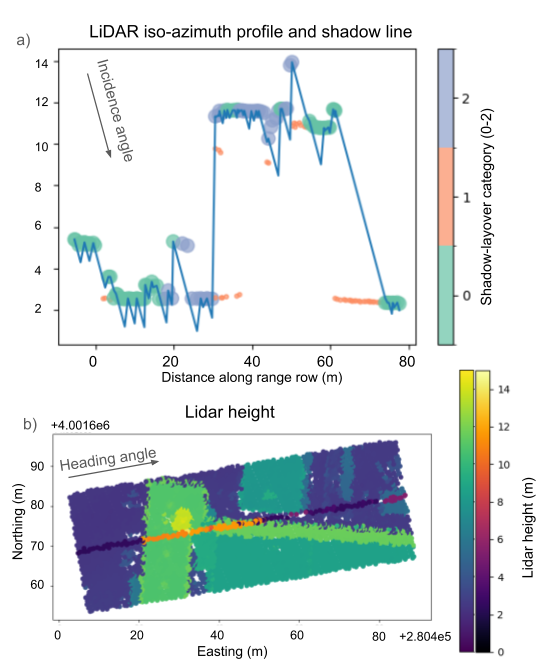
\includegraphics[width=\linewidth,height=0.68\textheight,keepaspectratio]{figures/ch3_shadow_profile.png}
  \end{columns}
\end{frame}

\begin{frame}{Espacio blanqueado}
  \begin{itemize}
    \item La incertidumbre posicional InSAR no es isotropa.
    \item Se modela en \texttt{RAC} y se transforma a \texttt{ENU}.
    \item La vinculacion se hace por plausibilidad geometrica, no por distancia euclidea simple.
  \end{itemize}
\end{frame}

\begin{frame}{Resultado global: distancia blanqueada}
  \begin{columns}[T,totalwidth=\textwidth]
    \column{0.49\textwidth}
    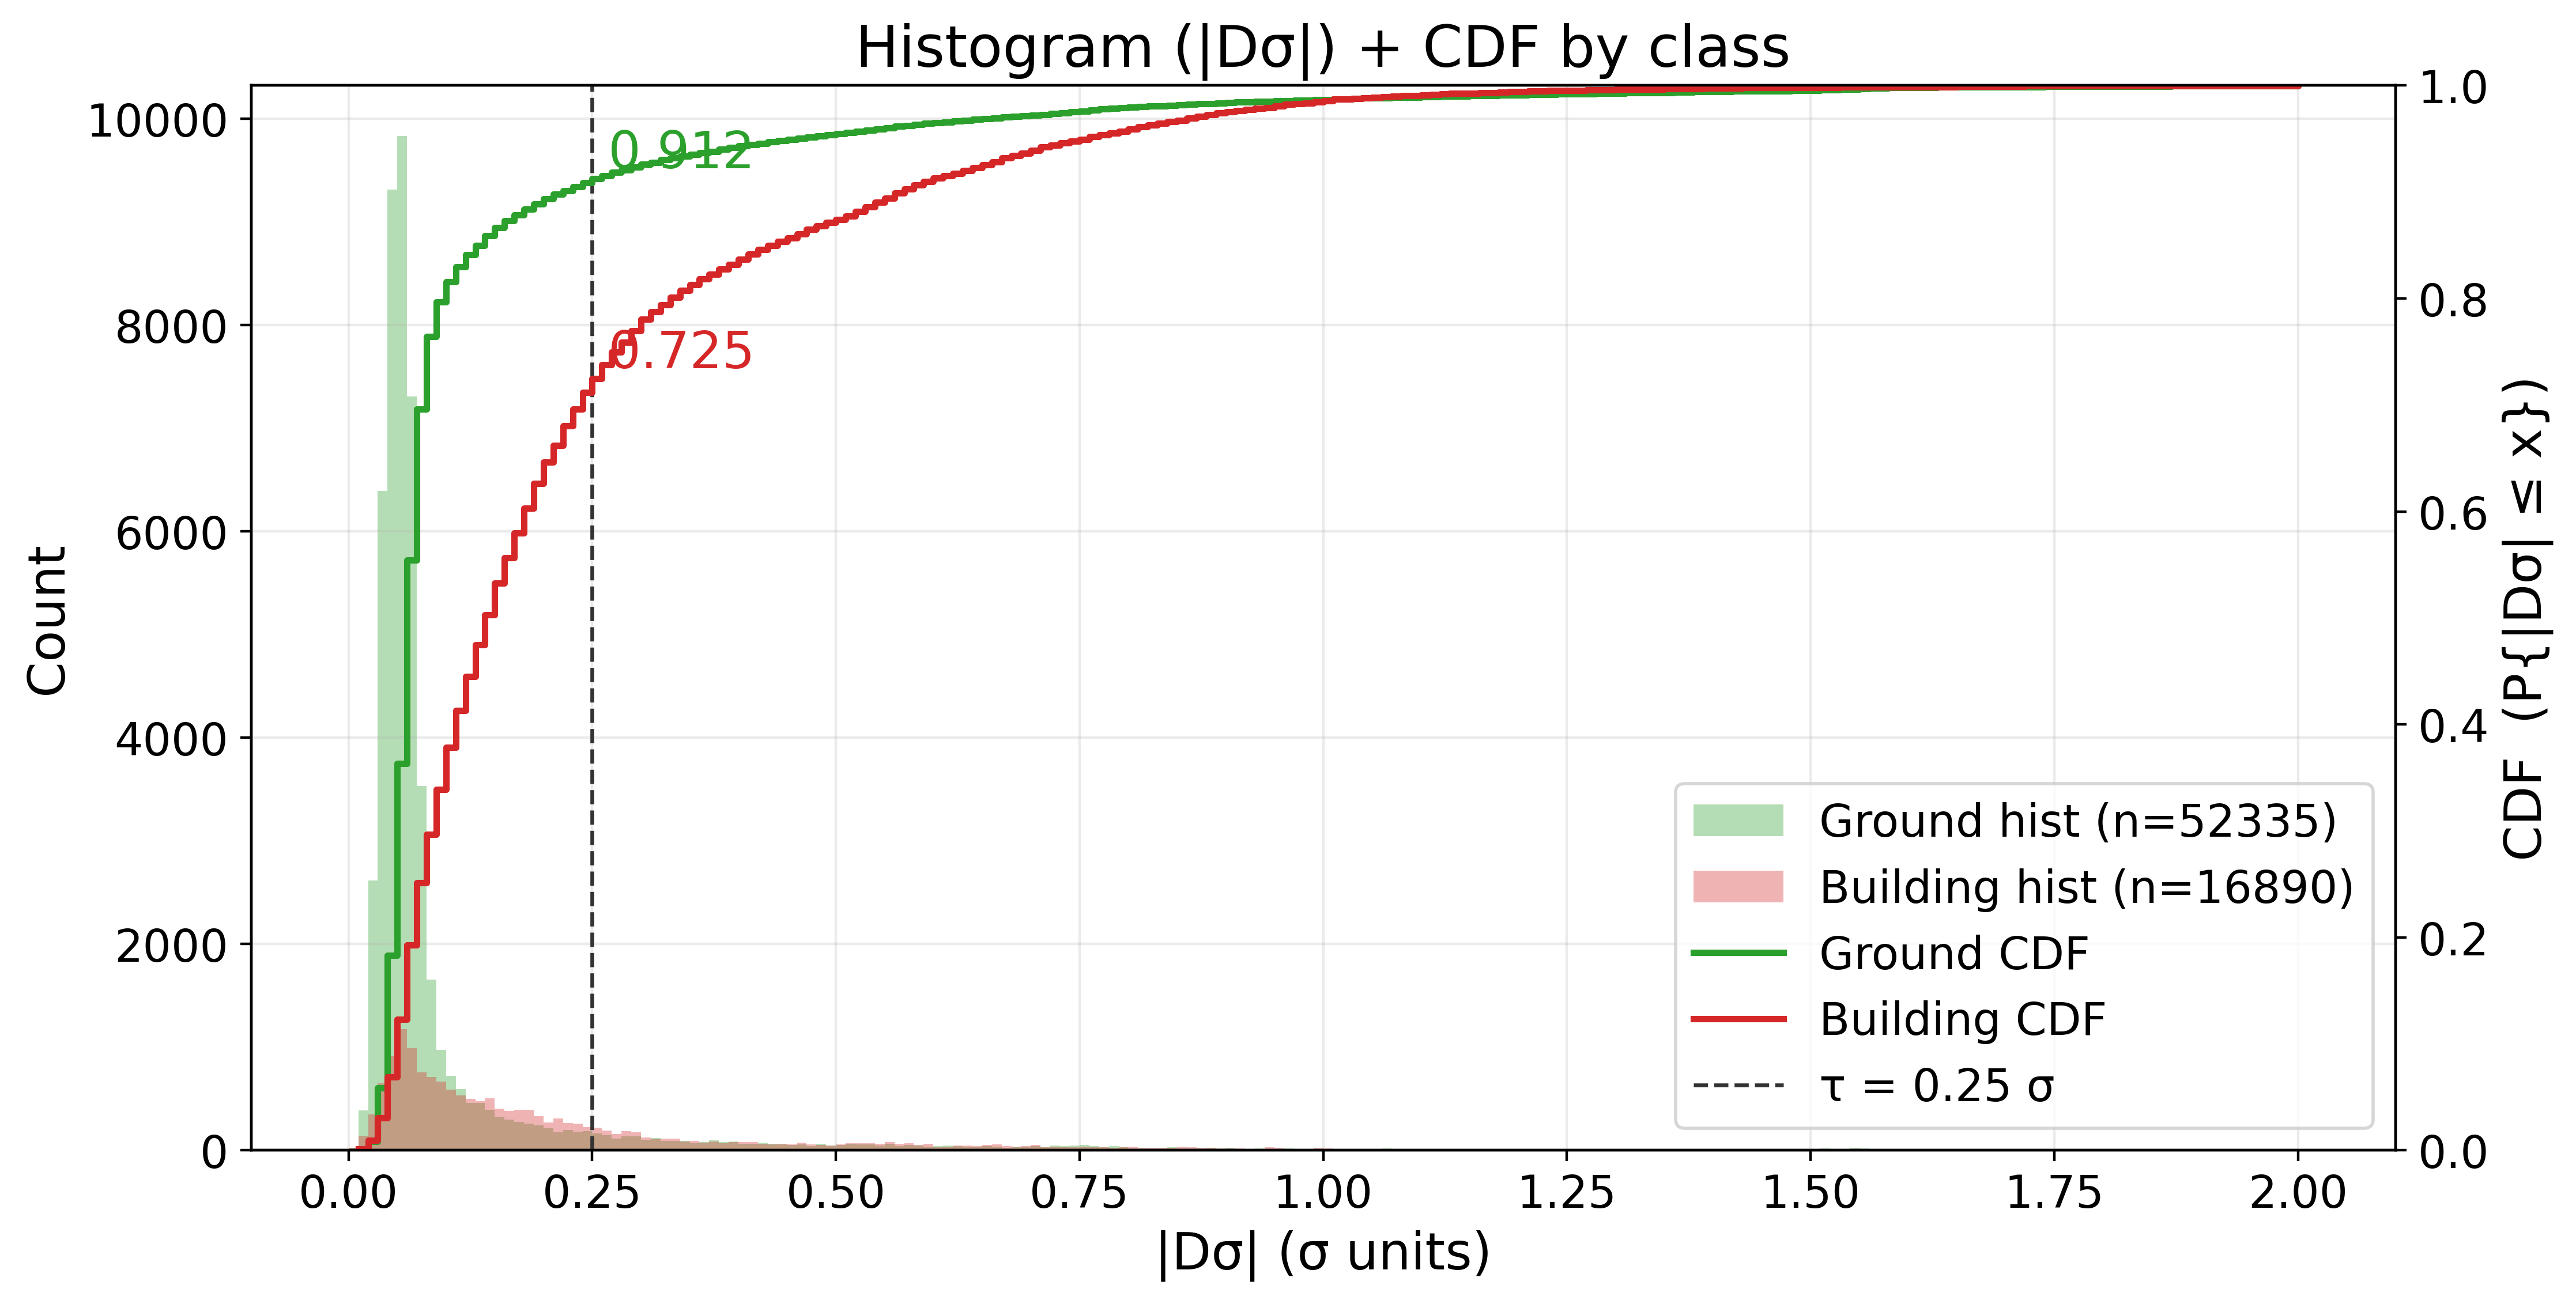
\includegraphics[width=\linewidth]{figures/ch3_sl_sigma_asc.png}
    \column{0.49\textwidth}
    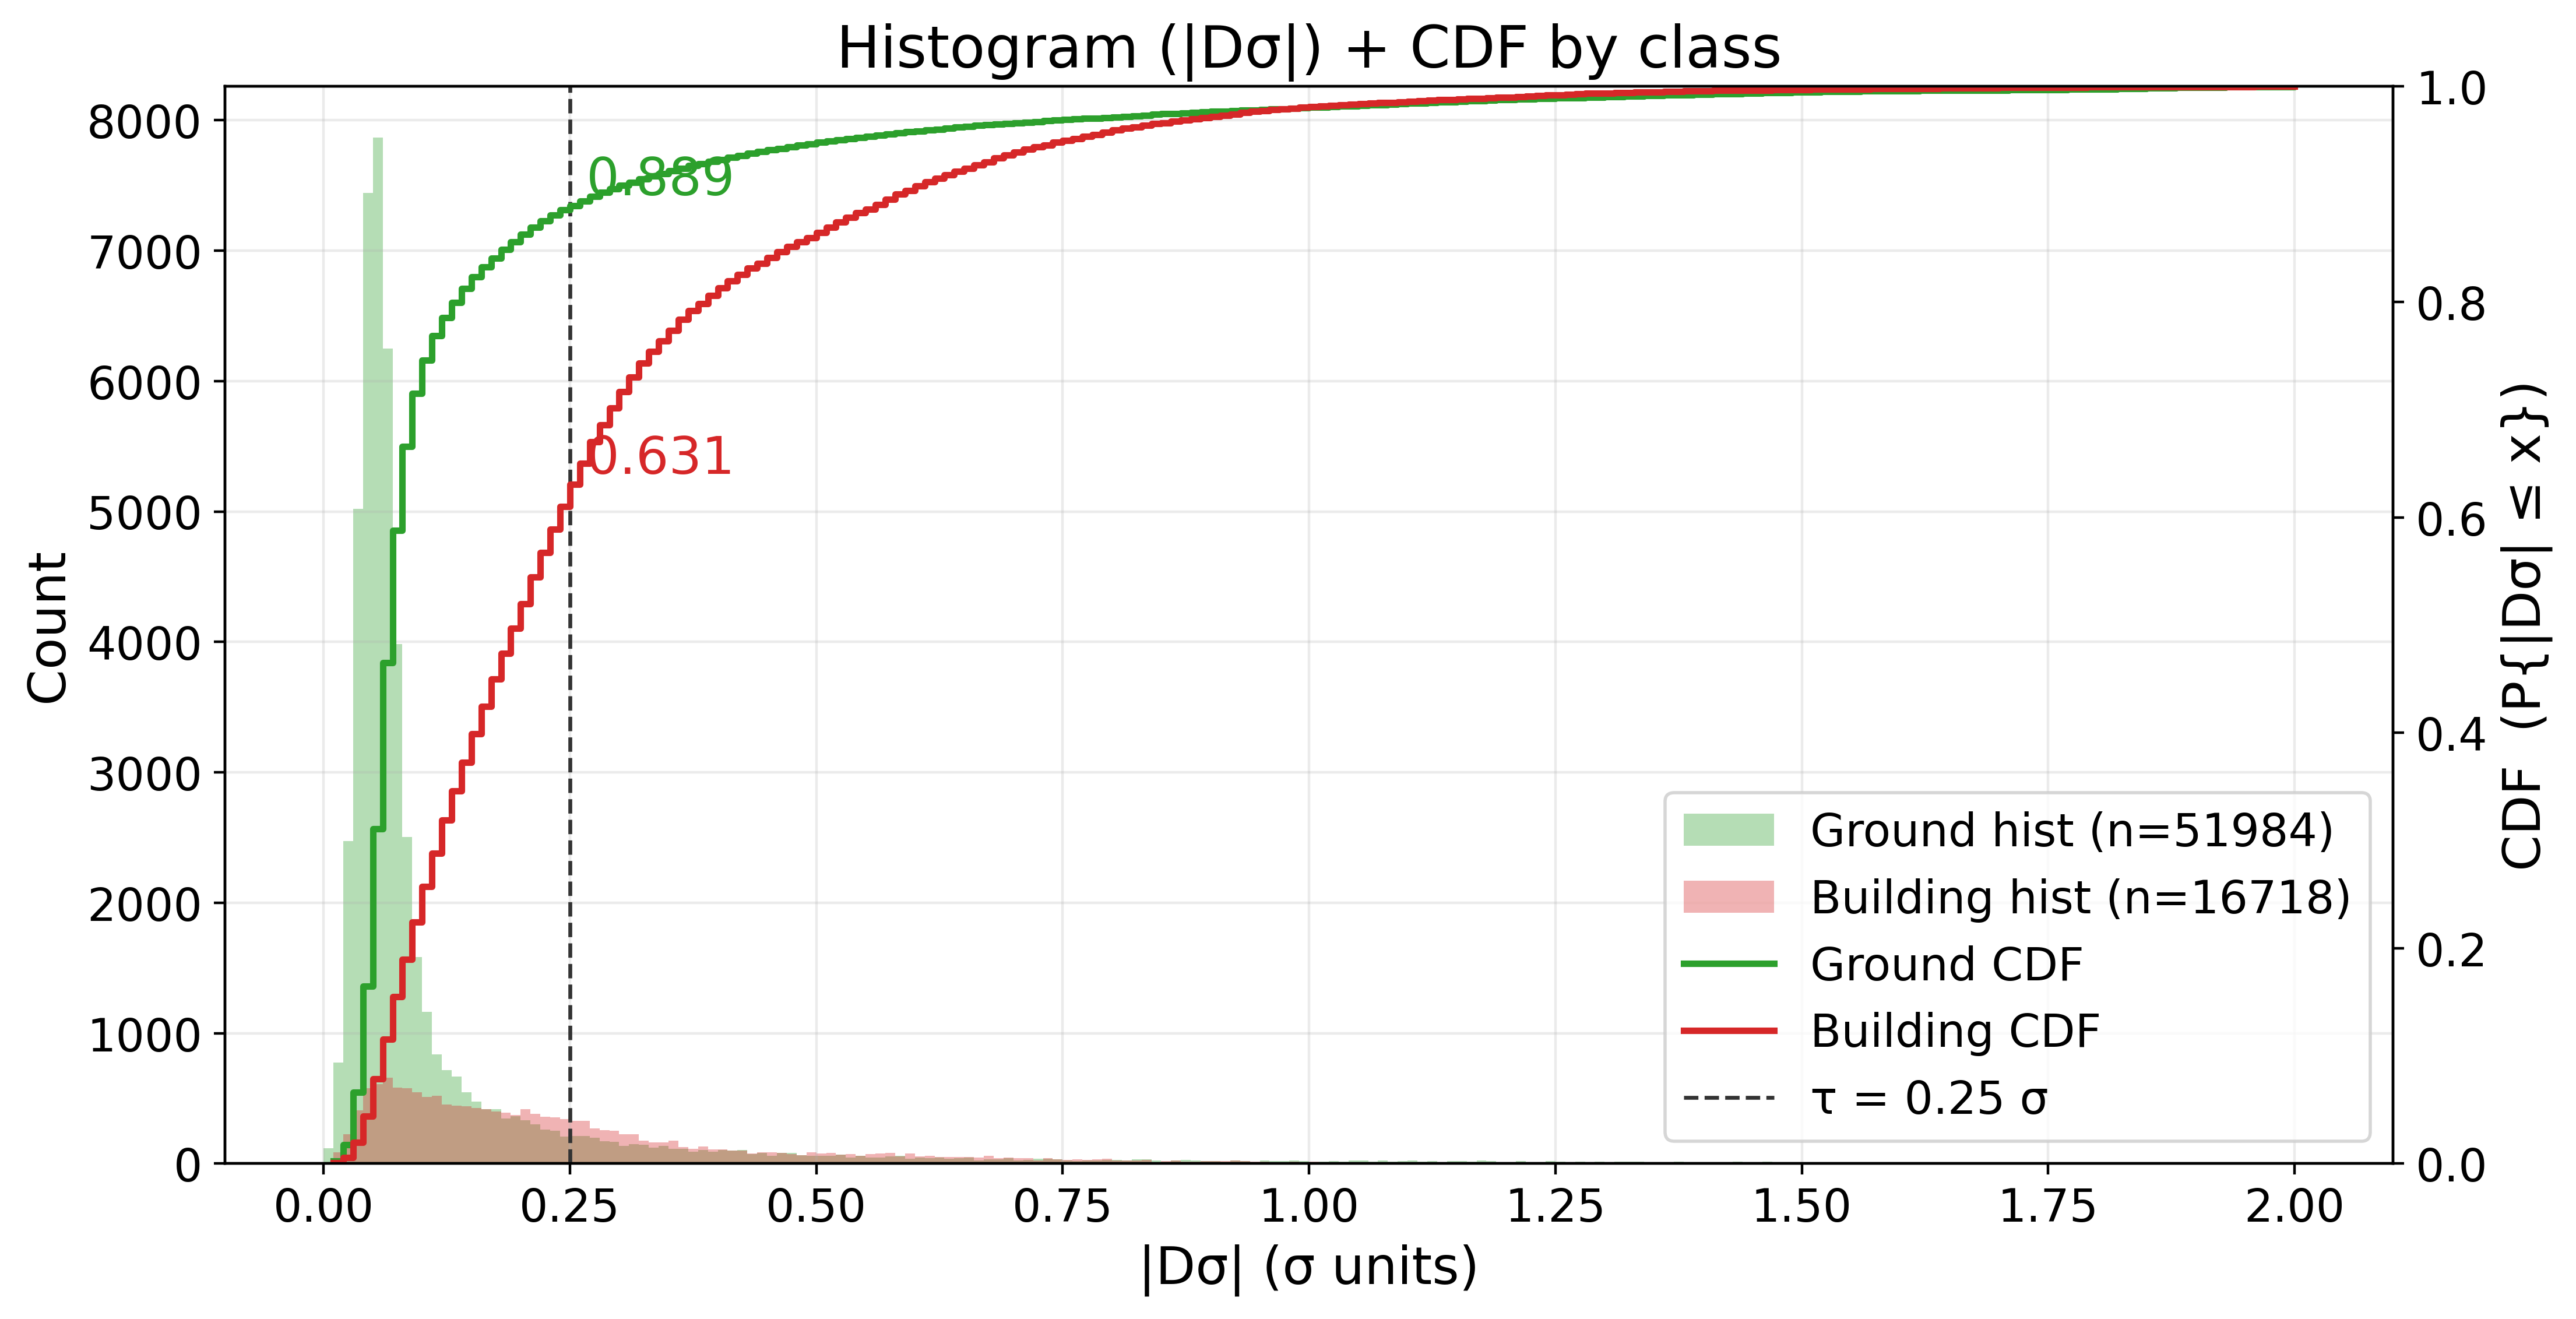
\includegraphics[width=\linewidth]{figures/ch3_sl_sigma_dsc.png}
  \end{columns}
\end{frame}

\begin{frame}{Resultado 3D: tanques}
  \centering
  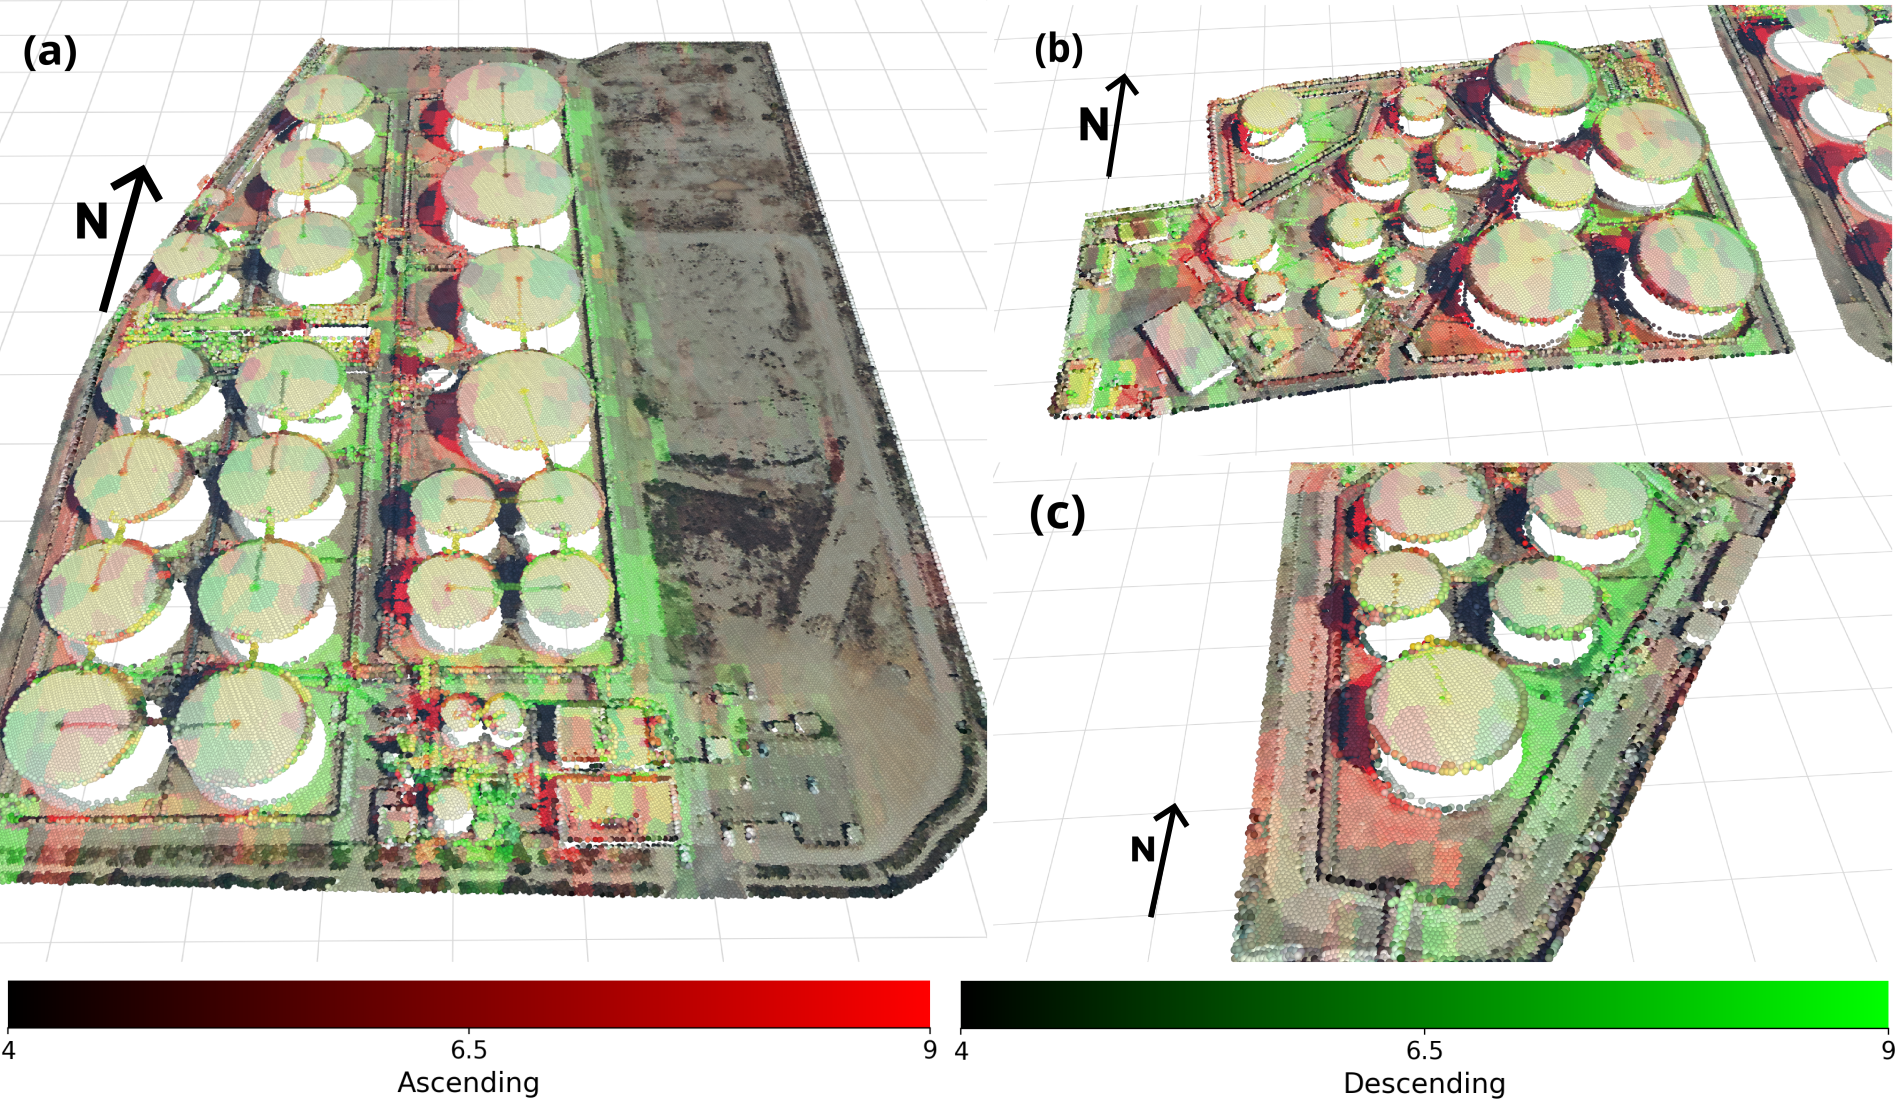
\includegraphics[width=0.95\linewidth,height=0.76\textheight,keepaspectratio]{figures/ch3_tanks_rgb.png}
\end{frame}

\begin{frame}{Resultado 3D: EVOS}
  \centering
  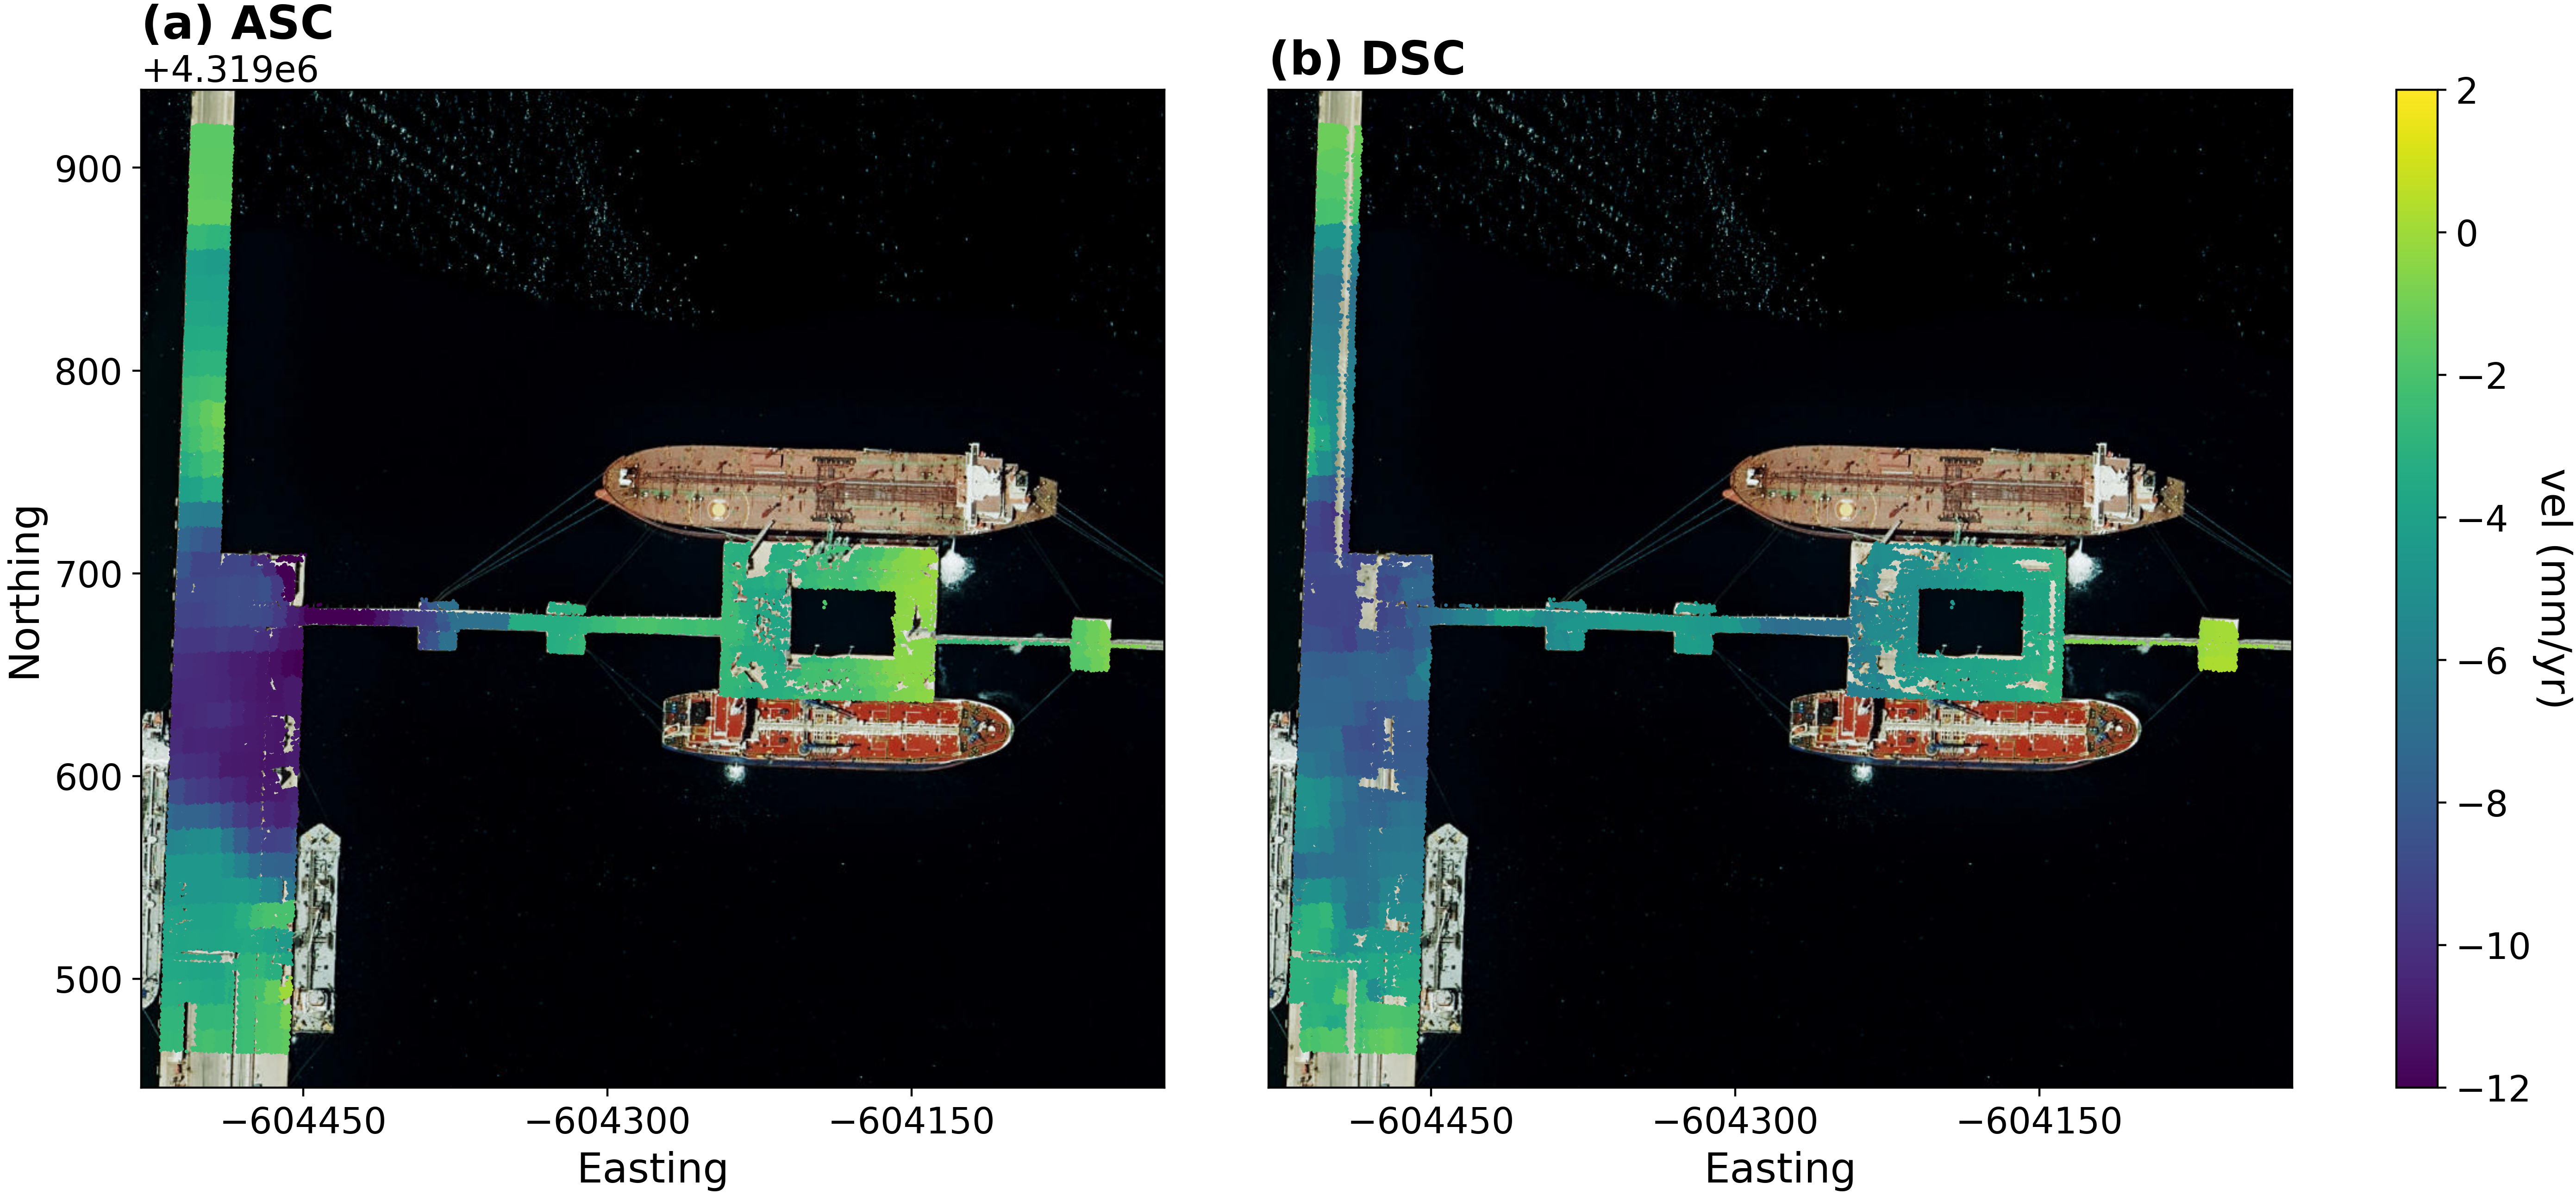
\includegraphics[width=0.92\linewidth]{figures/ch3_evos_vel.png}
\end{frame}

\begin{frame}{Mensaje del capitulo 3}
  \begin{itemize}
    \item La observacion solo se vuelve accionable cuando queda bien atribuida.
    \item La incertidumbre no es solo espacial: es geometrica y dependiente del activo.
    \item InSAR gana valor de ingenieria al anclarse a la nube LiDAR y al activo real.
  \end{itemize}
\end{frame}

\section{Capitulo 4: Interpretacion}

\begin{frame}{Capitulo 4: el problema interpretativo}
  \begin{itemize}
    \item No toda deformacion implica dano.
    \item Una velocidad lineal puede mezclar consolidacion, estacionalidad y cambios de regimen.
    \item Hace falta una lectura temporal mas rica y controlada estadisticamente.
  \end{itemize}
\end{frame}

\begin{frame}{Por que MHT}
  \begin{itemize}
    \item \textbf{Multiple Hypothesis Testing} compara hipotesis fisicas en competencia.
    \item Permite detectar offsets, estacionalidad y cambios de regimen.
    \item Evita depender de umbrales genericos y fragiles.
    \item Hipotesis nula: comportamiento estacionario o tendencia simple.
    \item Hipotesis alternativas: termica, escalones, oleaje, no linealidades.
    \item Proceso DIA: deteccion, identificacion y adaptacion.
  \end{itemize}
\end{frame}

\begin{frame}{Metodo de Baarda}
  \begin{itemize}
    \item Compara modelos de distinta complejidad de manera justa.
    \item No selecciona un modelo mas complejo salvo que haya evidencia suficiente.
    \item Es clave para reducir falsas alarmas en contexto portuario.
  \end{itemize}
\end{frame}

\begin{frame}{VAI y metricas}
  \begin{itemize}
    \item El resultado final no es solo una serie temporal por punto.
    \item Se agregan metricas por \textbf{VAI}: \texttt{state}, \texttt{rate}, \texttt{offset}, \texttt{rate of change}, \texttt{Moran's I}.
    \item Asi se pasa de puntos a vigilancia por activos.
  \end{itemize}
\end{frame}

\begin{frame}{Casos de estudio del capitulo 4}
  \centering
  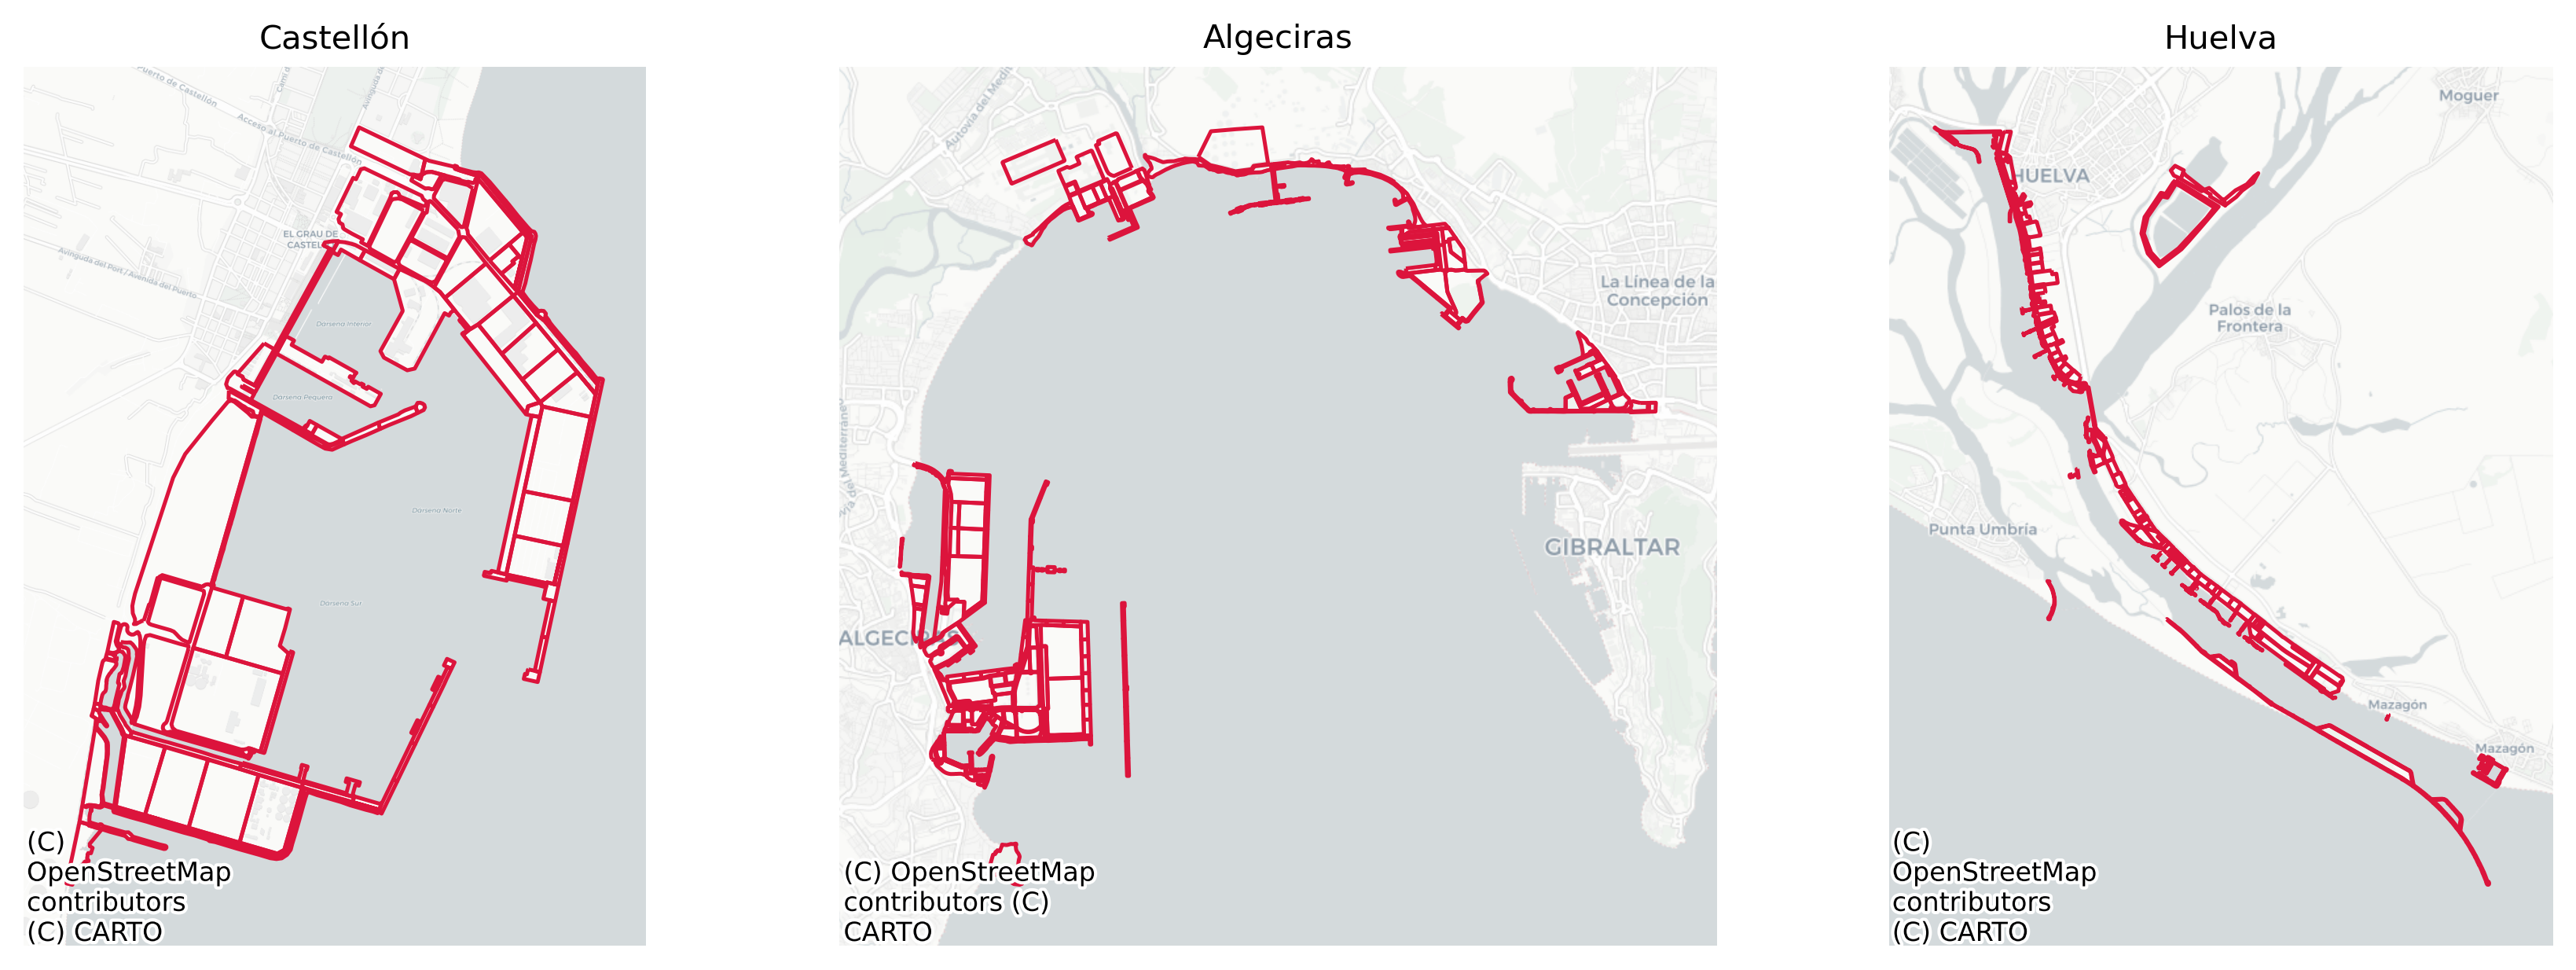
\includegraphics[width=0.82\linewidth]{figures/ch4_study_areas.png}
\end{frame}

\begin{frame}{Caso 1: Castellon y Storm Gloria}
  \centering
  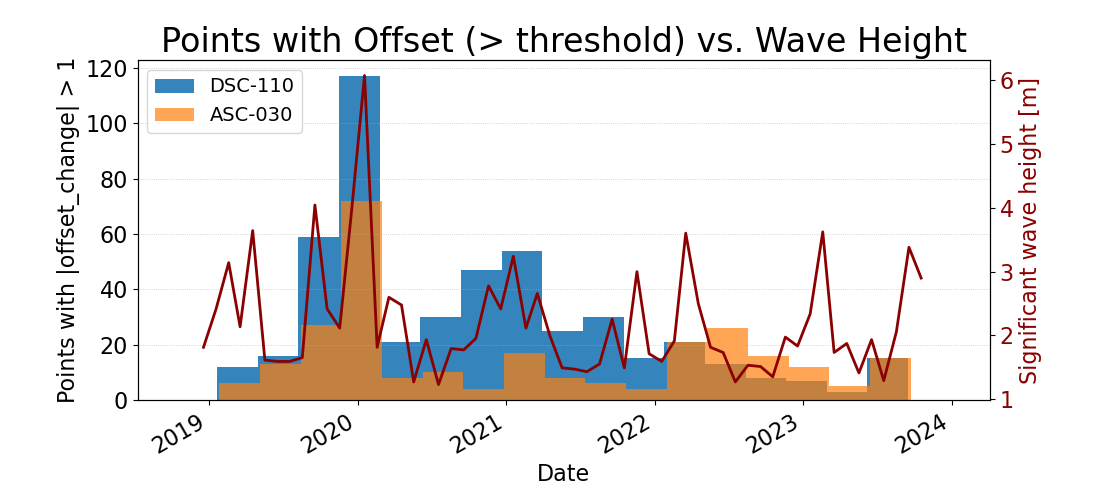
\includegraphics[width=0.92\linewidth]{figures/ch4_castellon_hist_offsets.png}
\end{frame}

\begin{frame}{Caso 1: huella espacial del evento}
  \begin{columns}[T,totalwidth=\textwidth]
    \column{0.49\textwidth}
    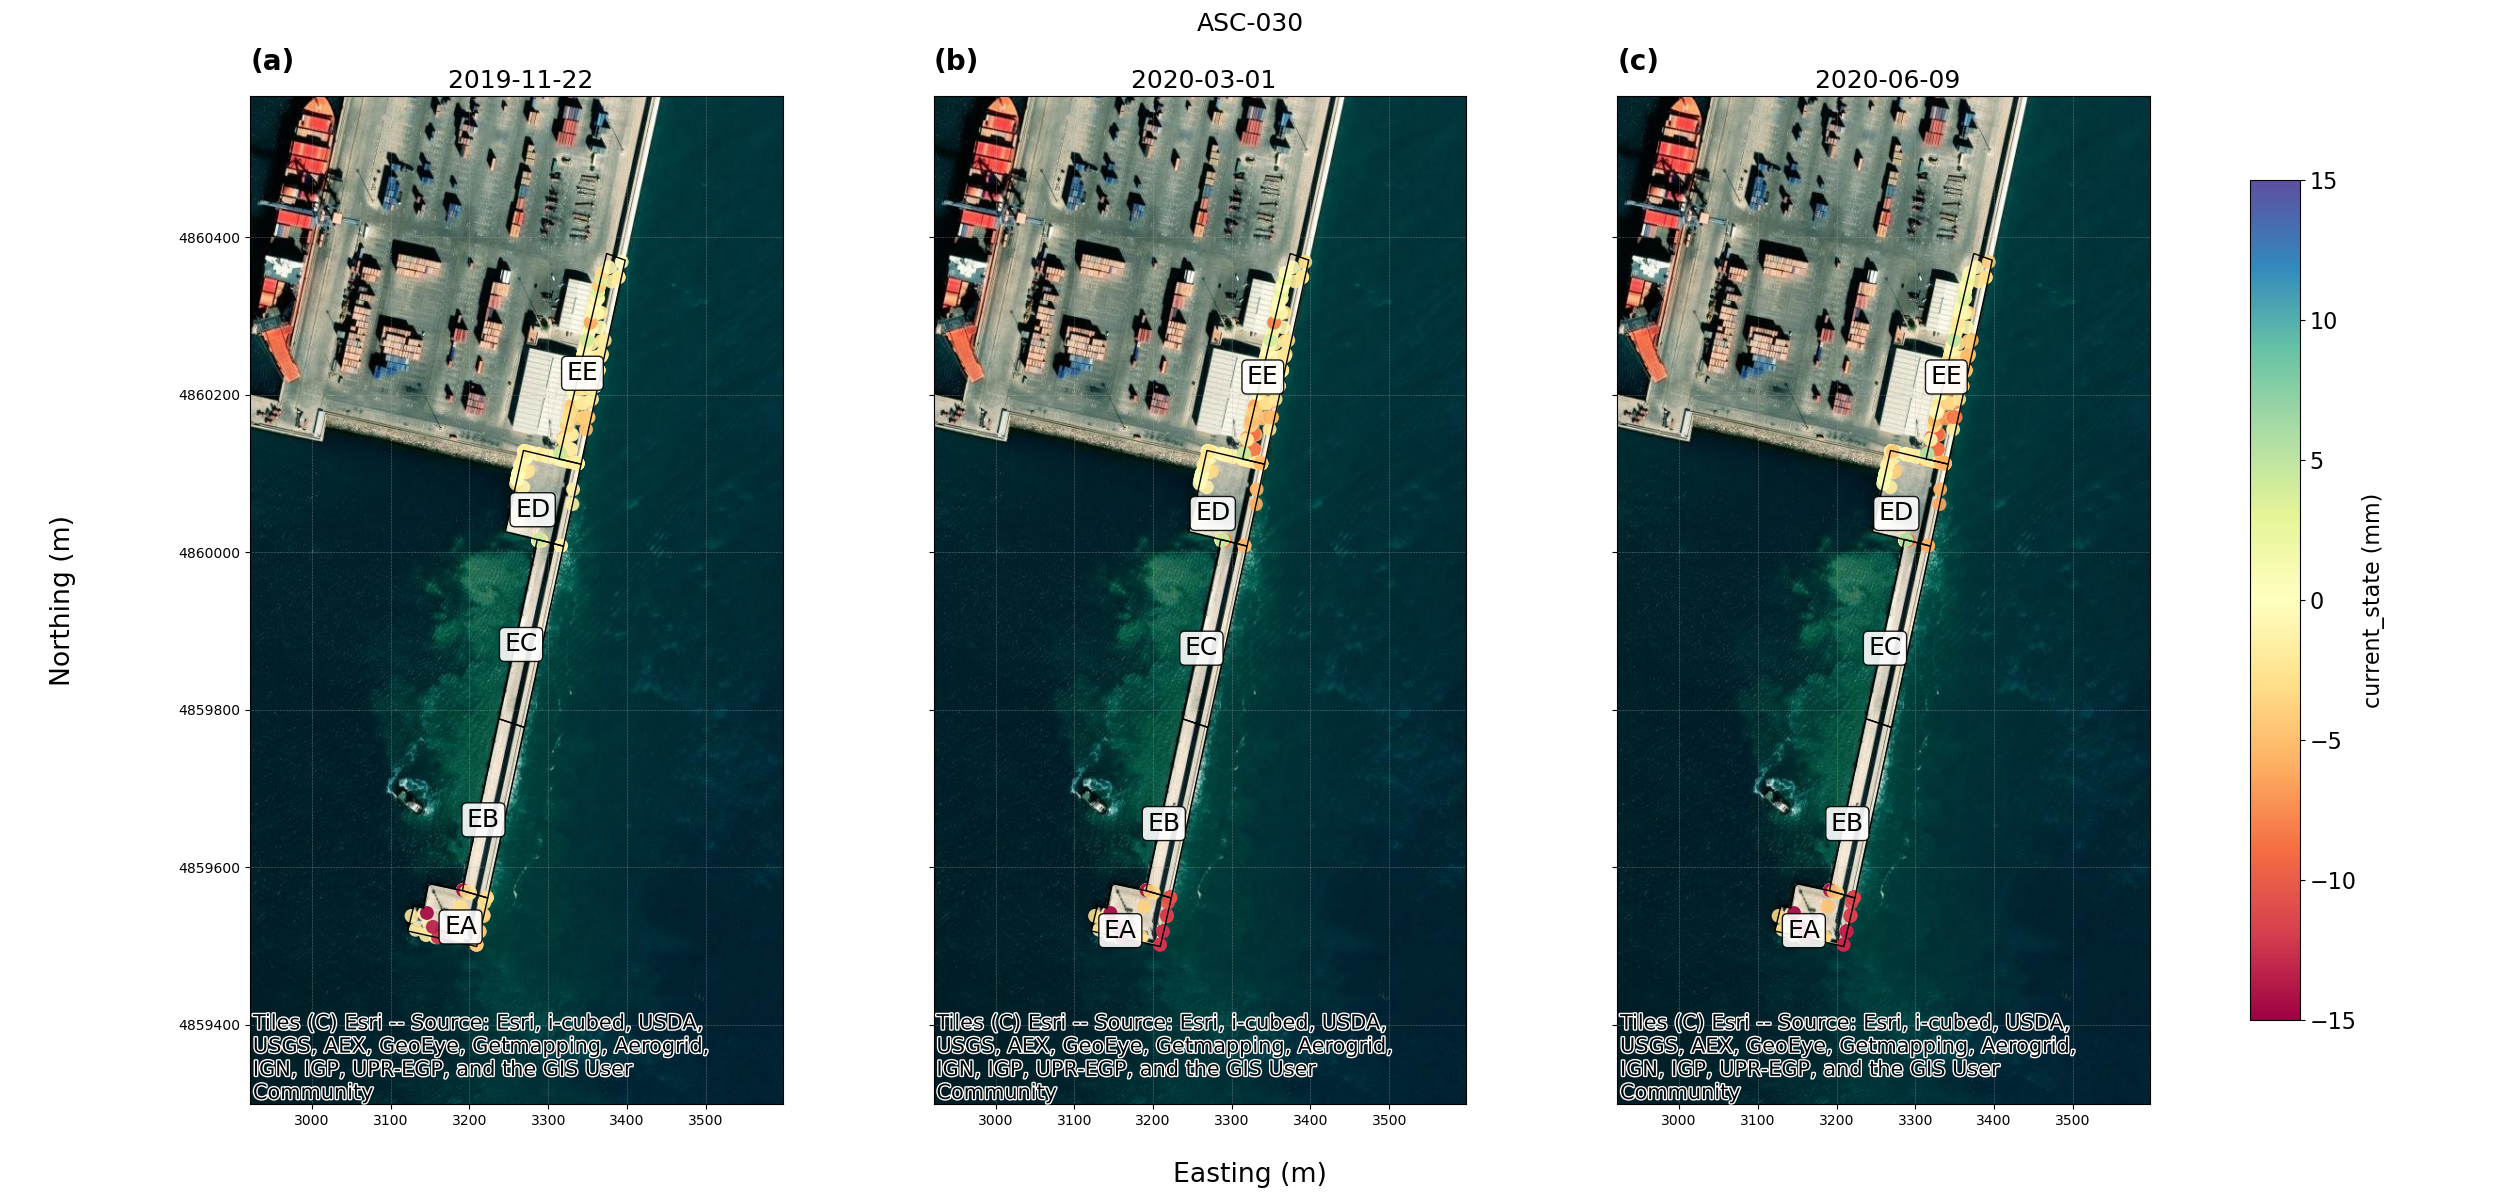
\includegraphics[width=\linewidth]{figures/ch4_castellon_spatial_1.png}
    \column{0.49\textwidth}
    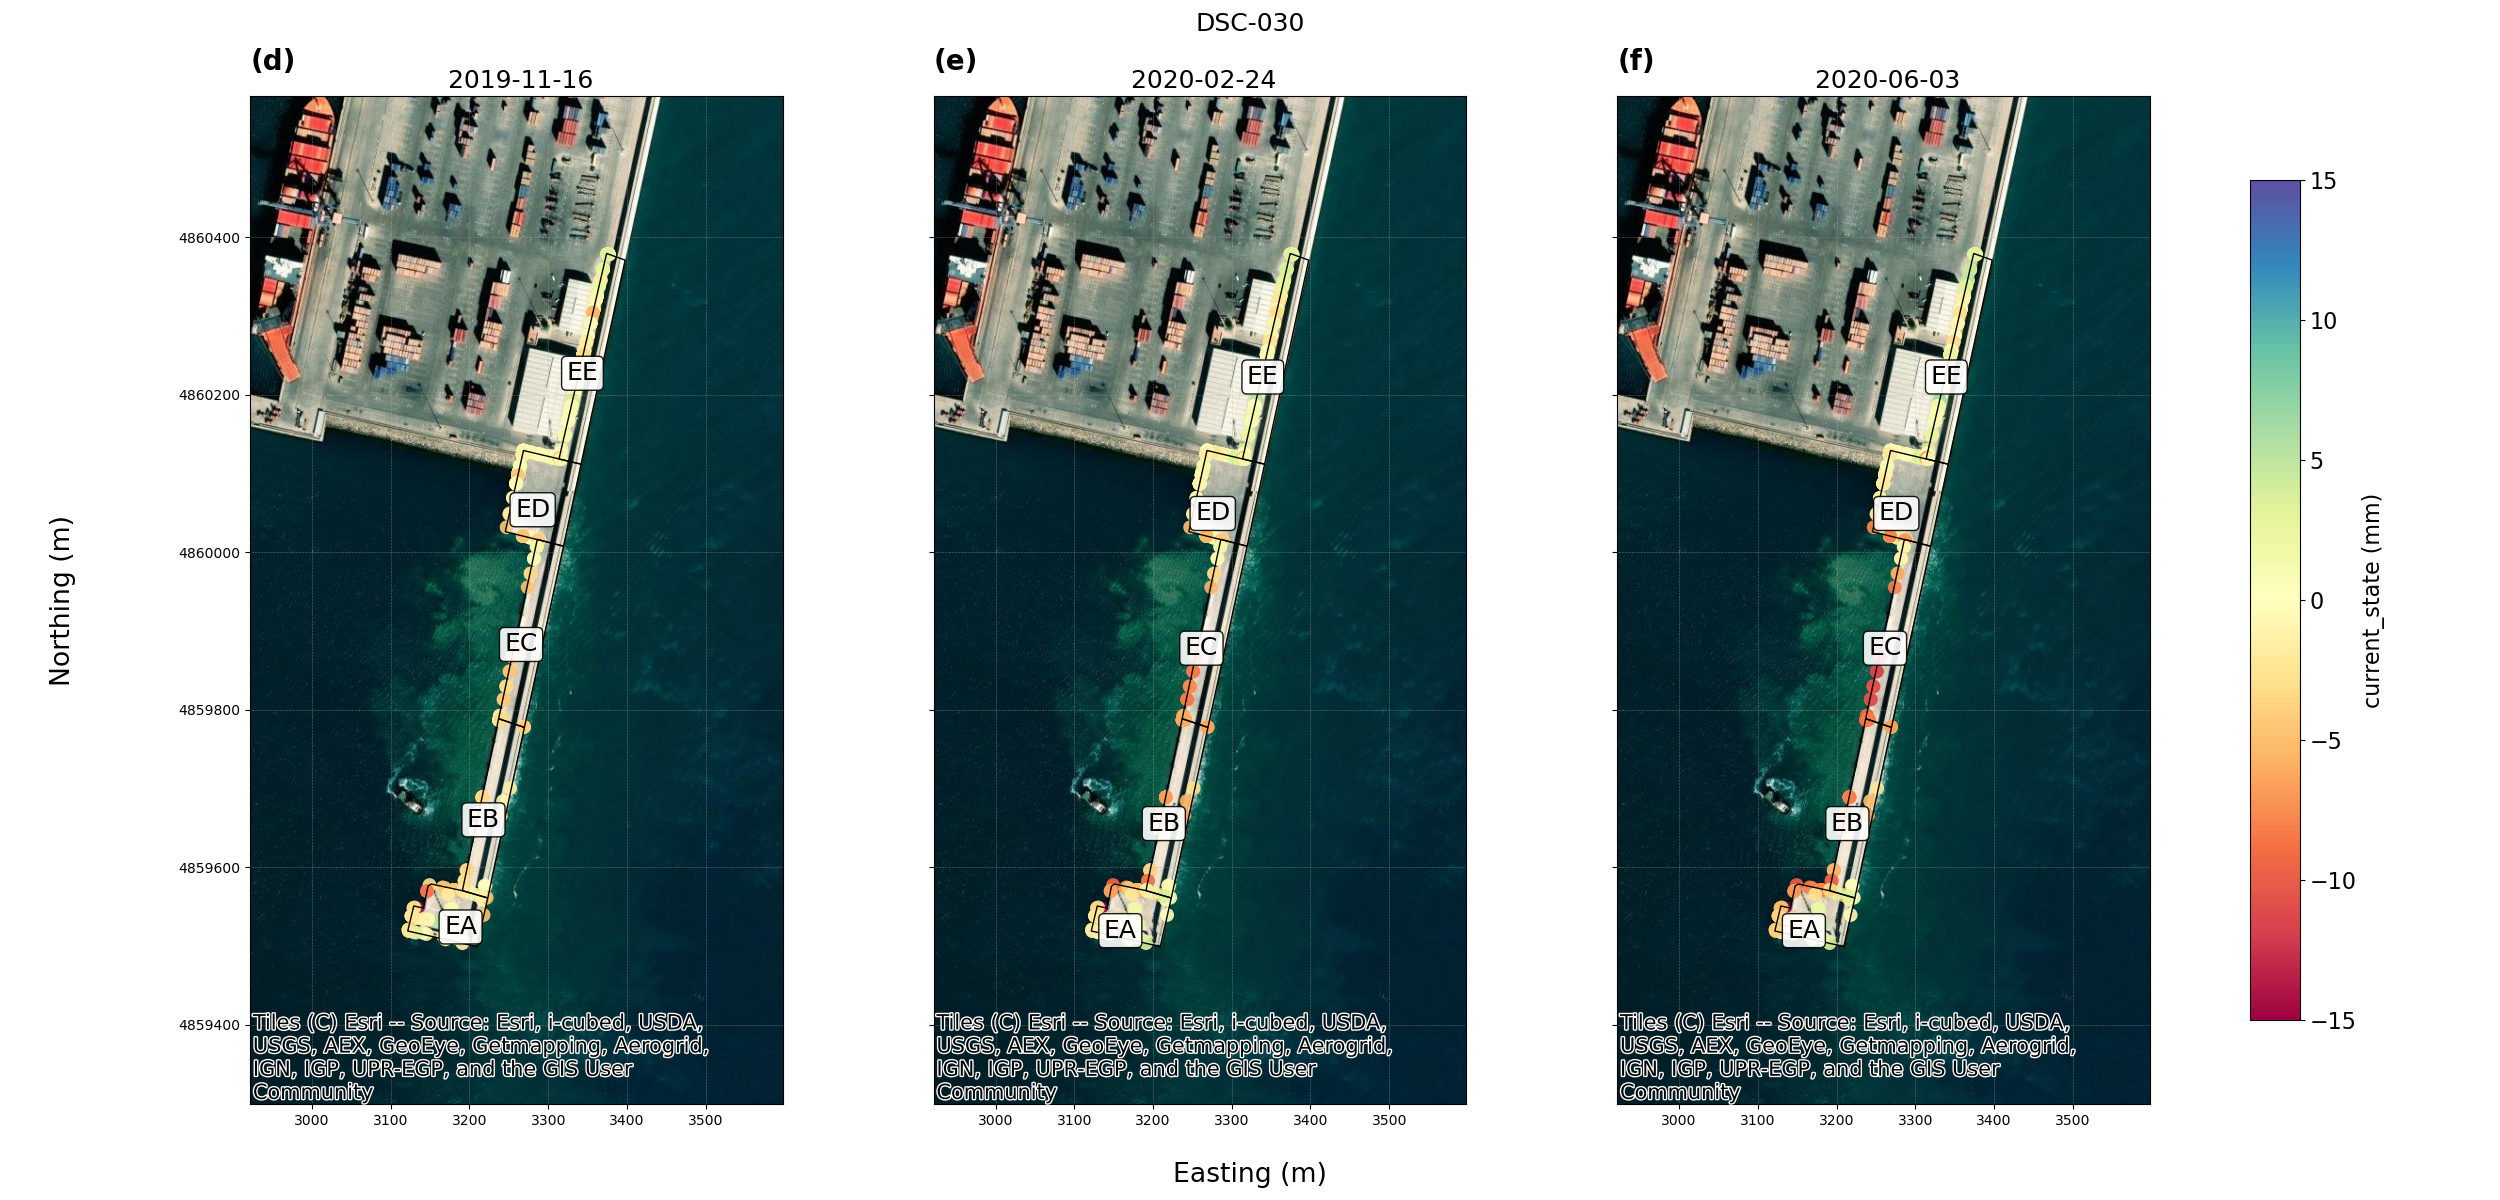
\includegraphics[width=\linewidth]{figures/ch4_castellon_spatial_2.png}
  \end{columns}
\end{frame}

\begin{frame}{Caso 2: Huelva y consolidacion coherente}
  \centering
  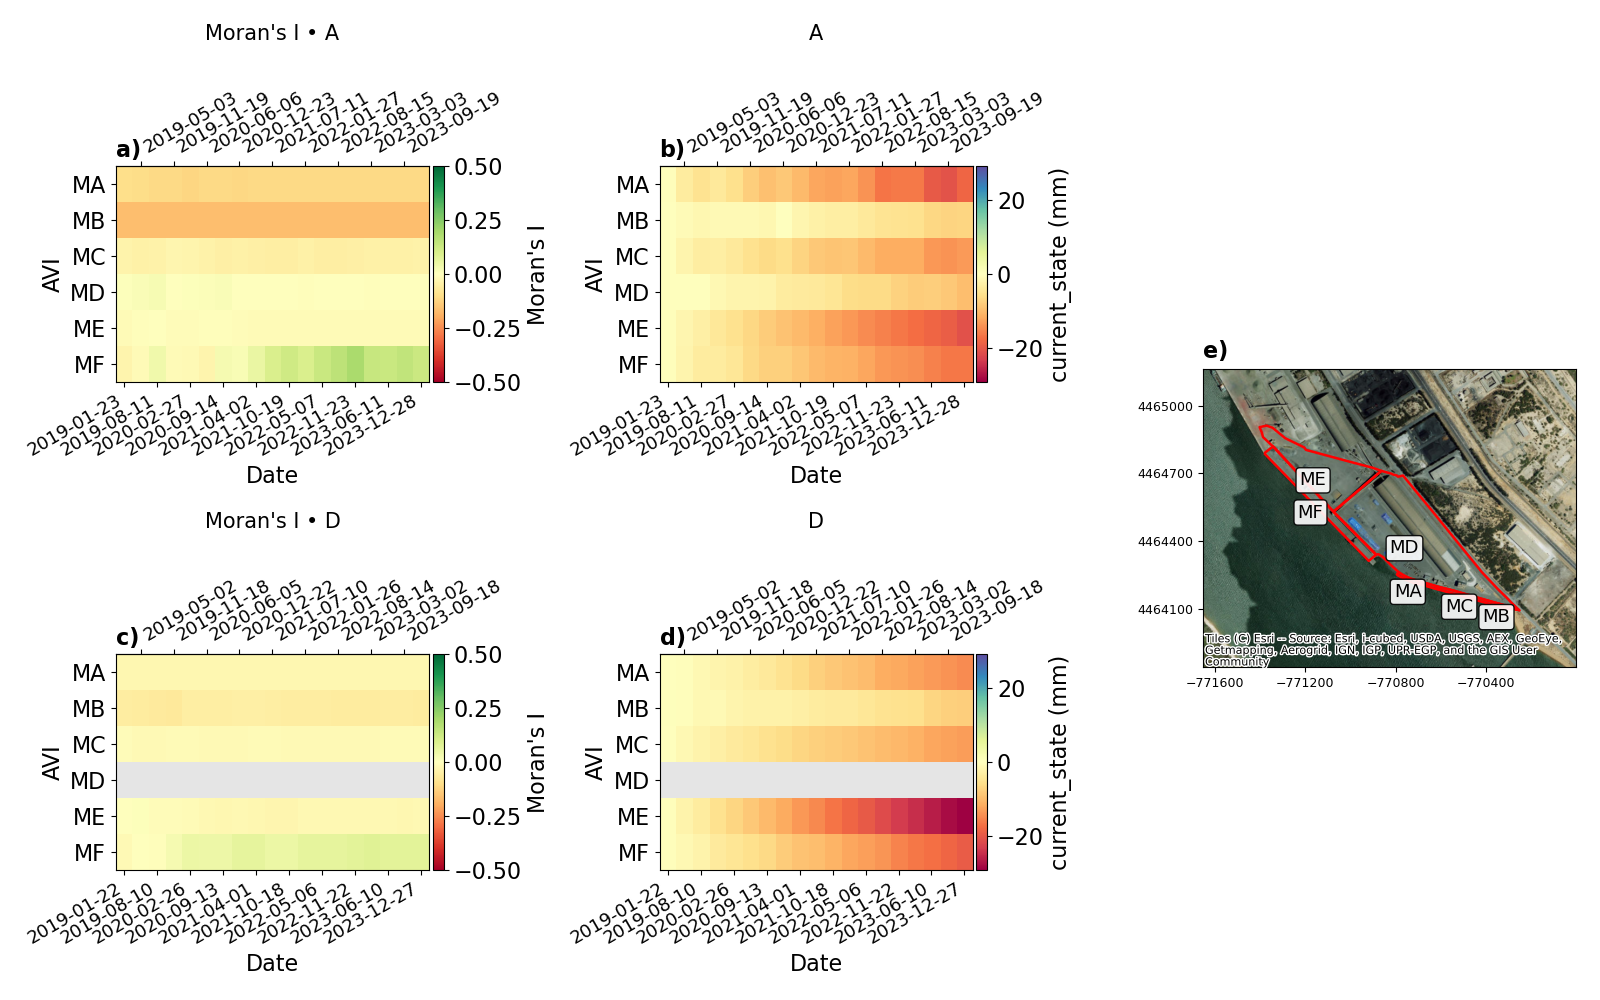
\includegraphics[width=0.92\linewidth,height=0.76\textheight,keepaspectratio]{figures/ch4_huelva_muelle_heatmap.png}
\end{frame}

\begin{frame}{Caso 2: Huelva y asentamiento diferencial}
  \begin{columns}[T,totalwidth=\textwidth]
    \column{0.49\textwidth}
    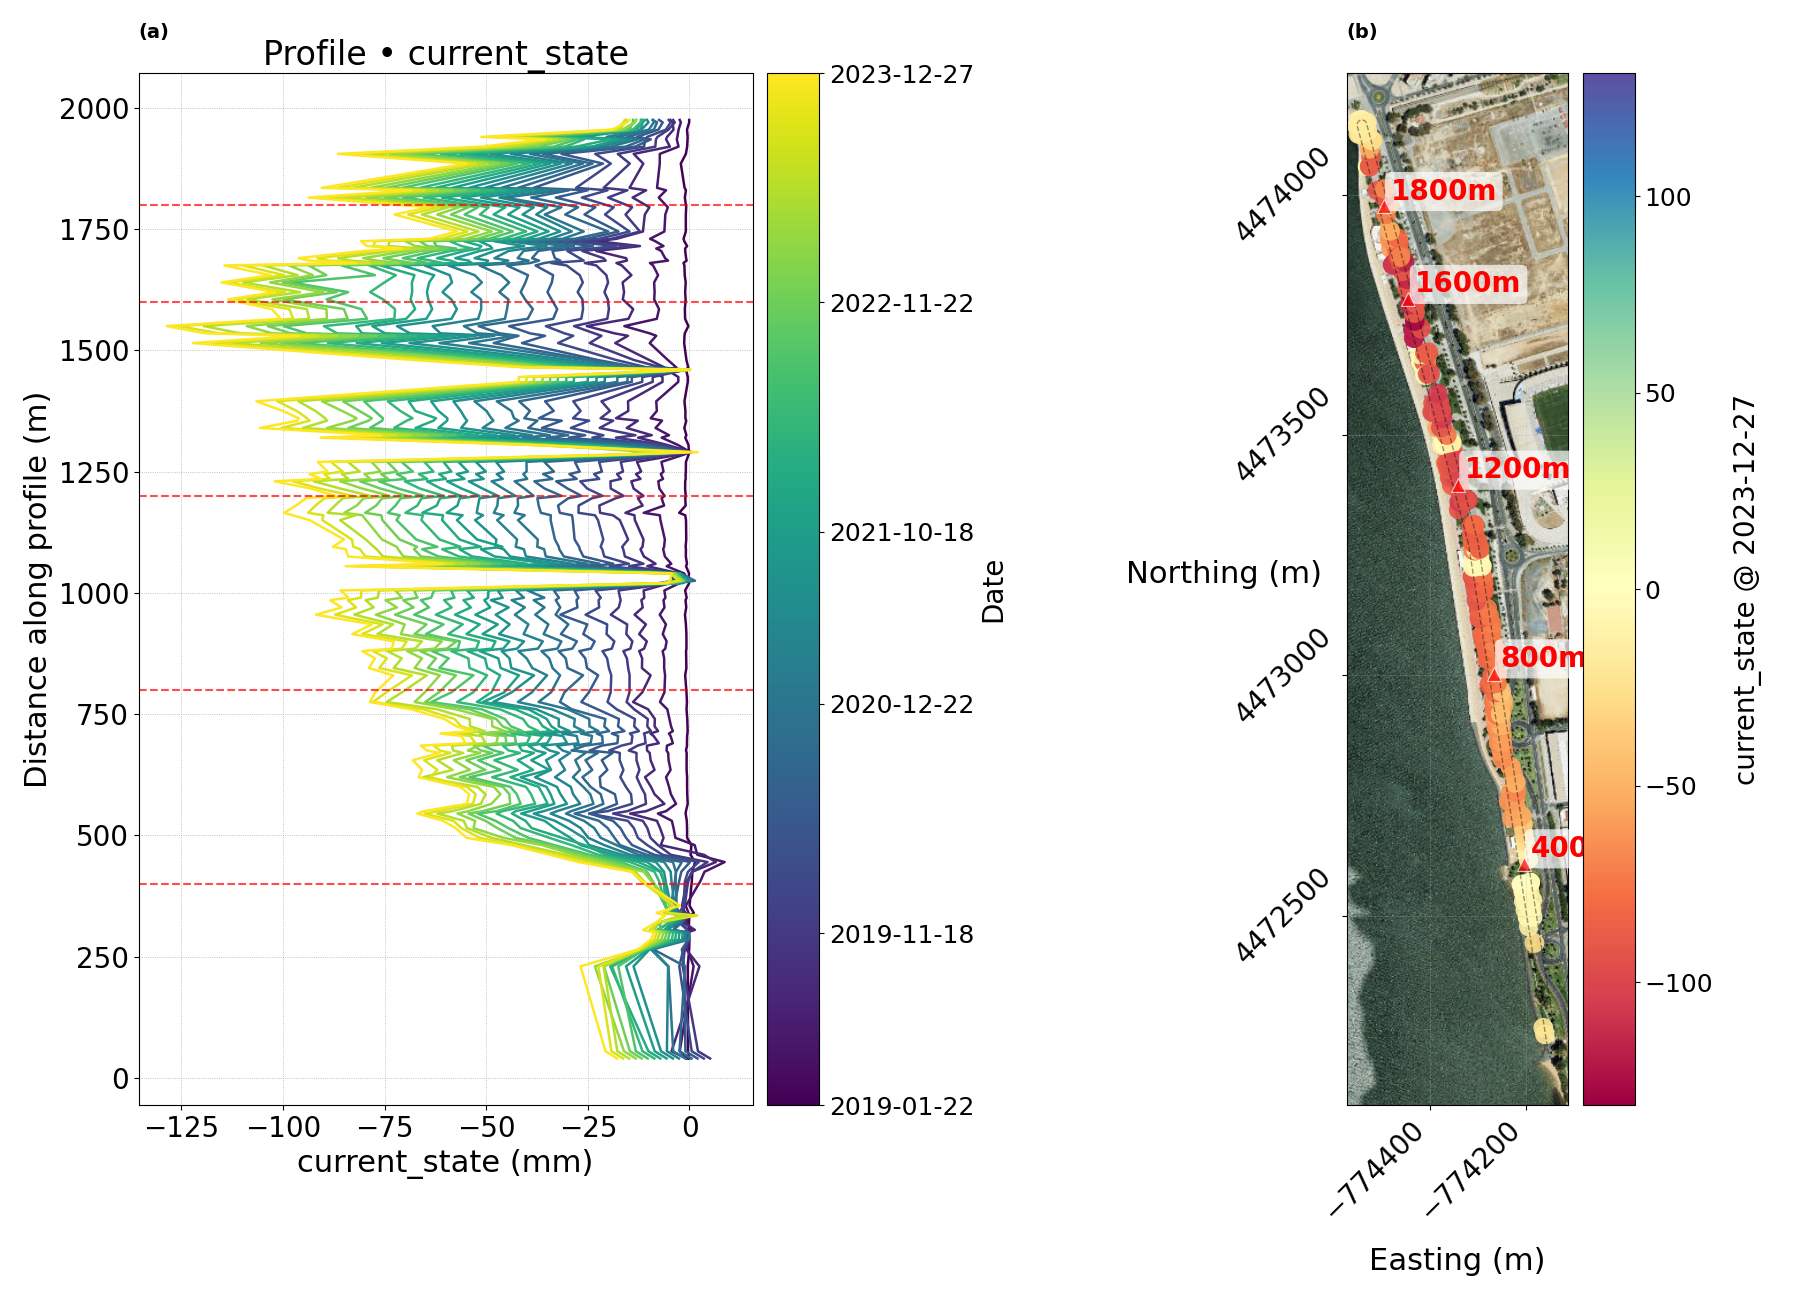
\includegraphics[width=\linewidth]{figures/ch4_huelva_paseo_profile_1.png}
    \column{0.49\textwidth}
    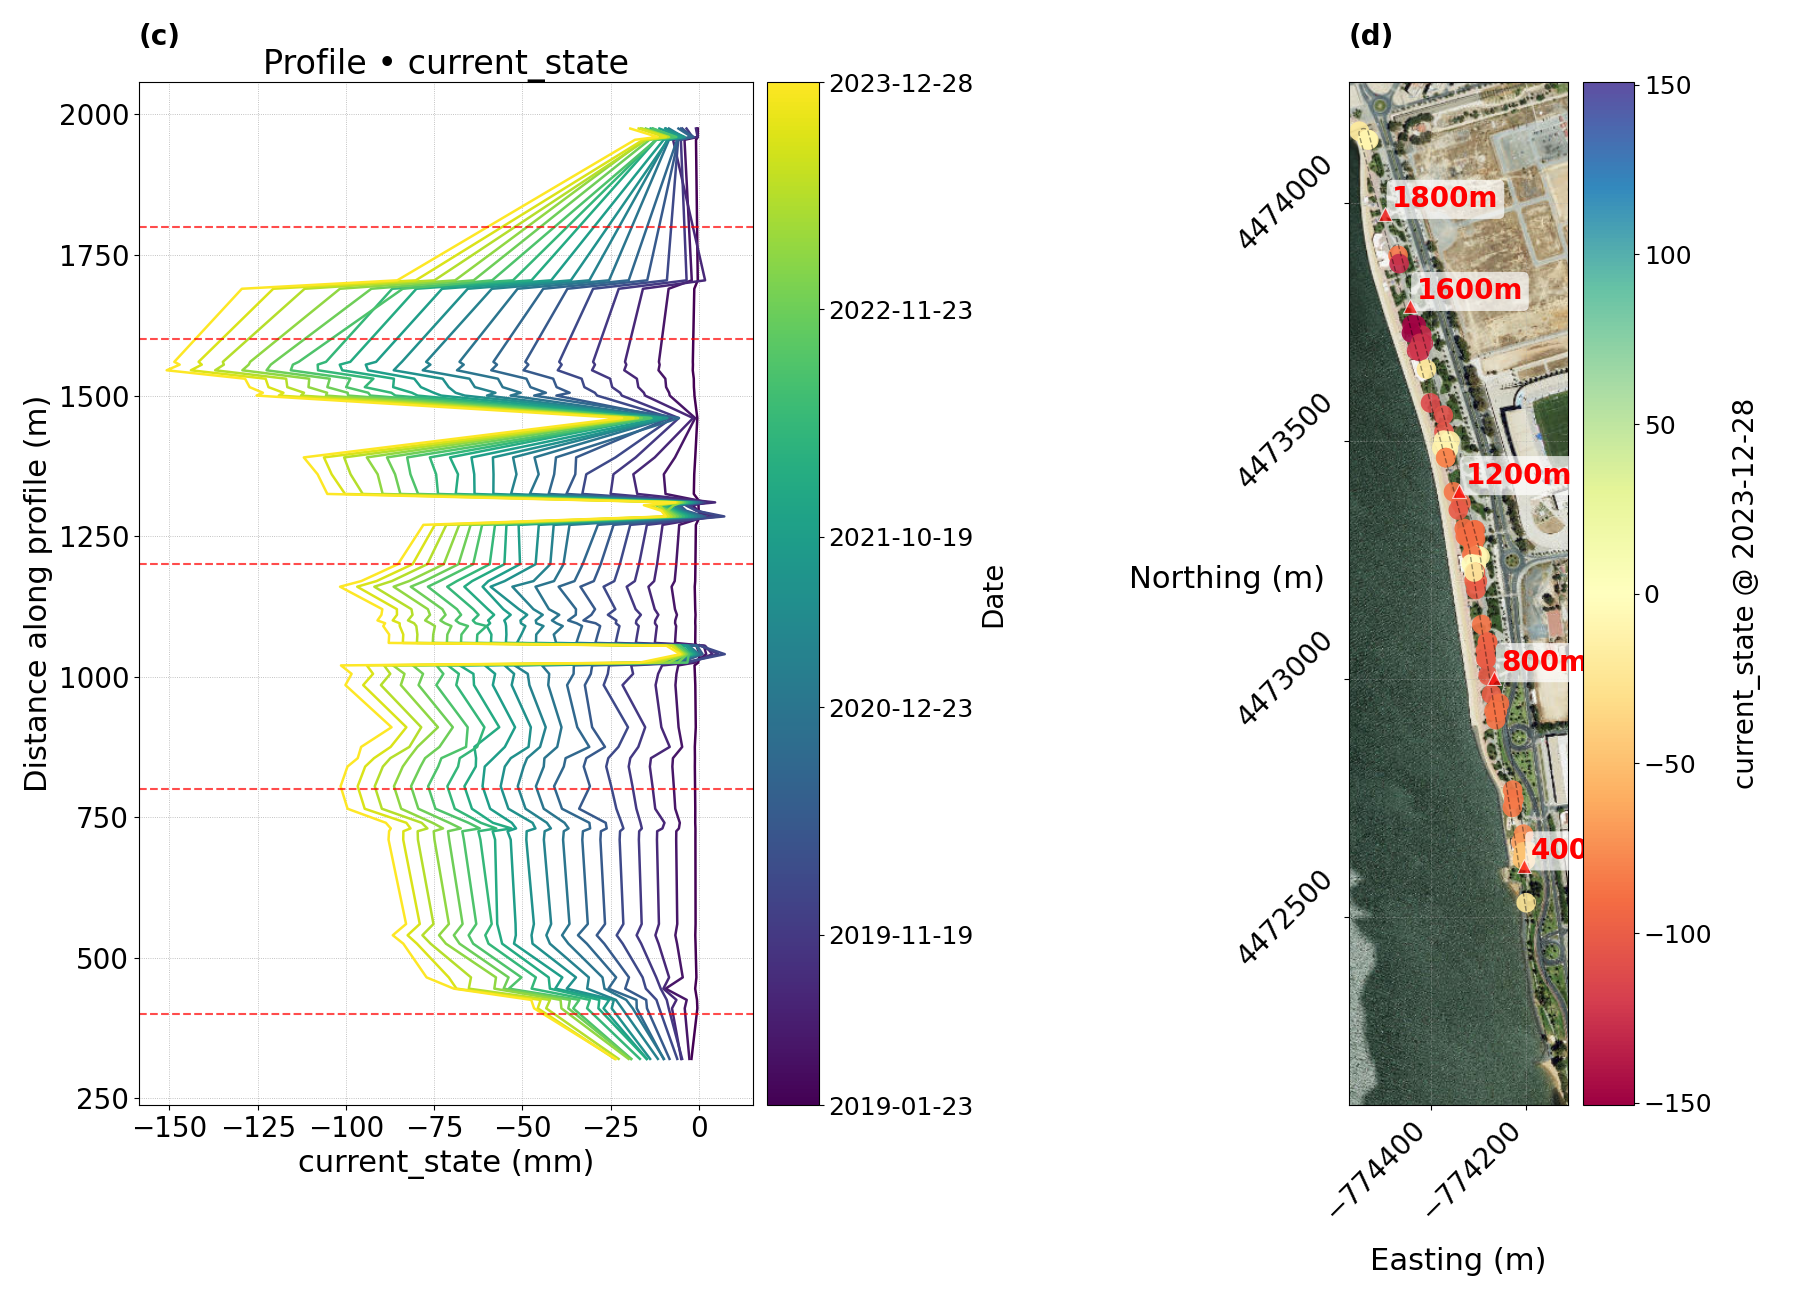
\includegraphics[width=\linewidth]{figures/ch4_huelva_paseo_profile_2.png}
  \end{columns}
\end{frame}

\begin{frame}{Caso 3: Algeciras y diagnostico multi-geometria}
  \begin{columns}[T,totalwidth=\textwidth]
    \column{0.49\textwidth}
    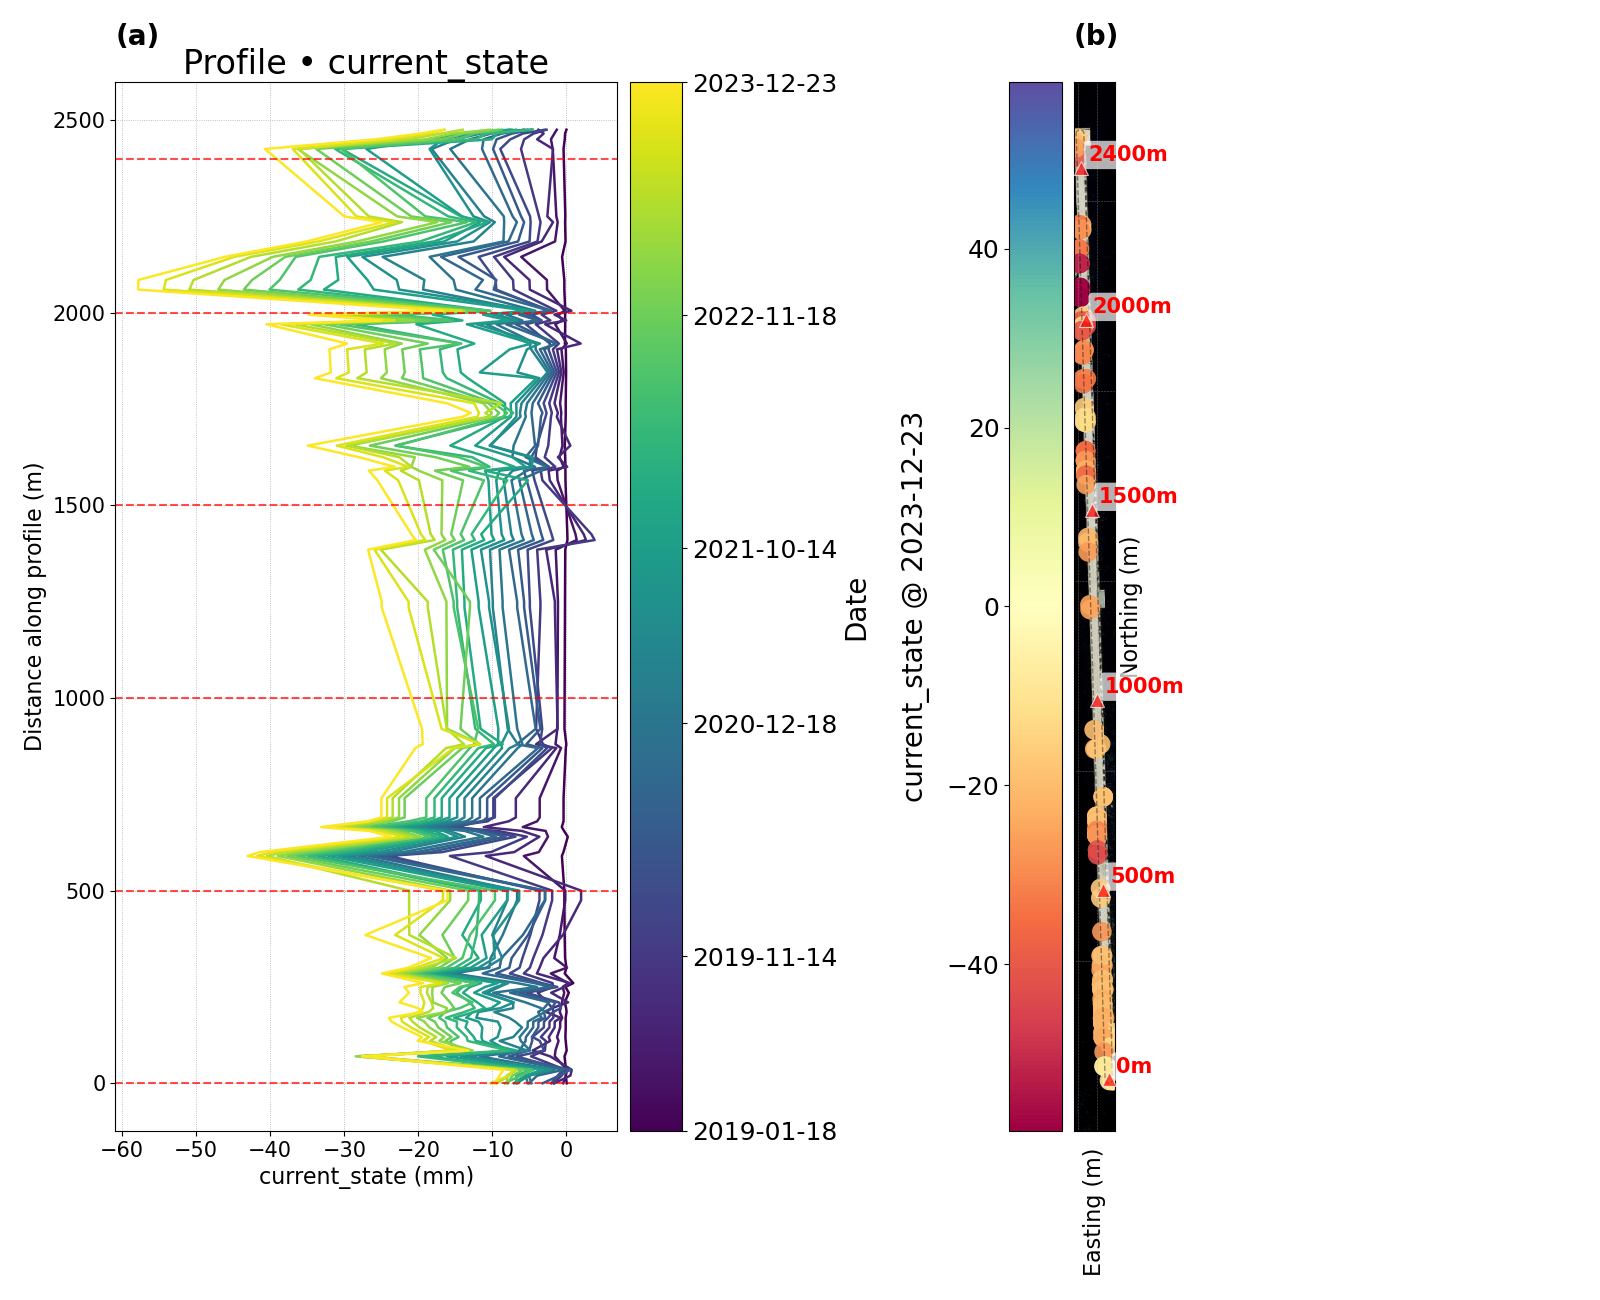
\includegraphics[width=\linewidth]{figures/ch4_algeciras_exento_profile_1.png}
    \column{0.49\textwidth}
    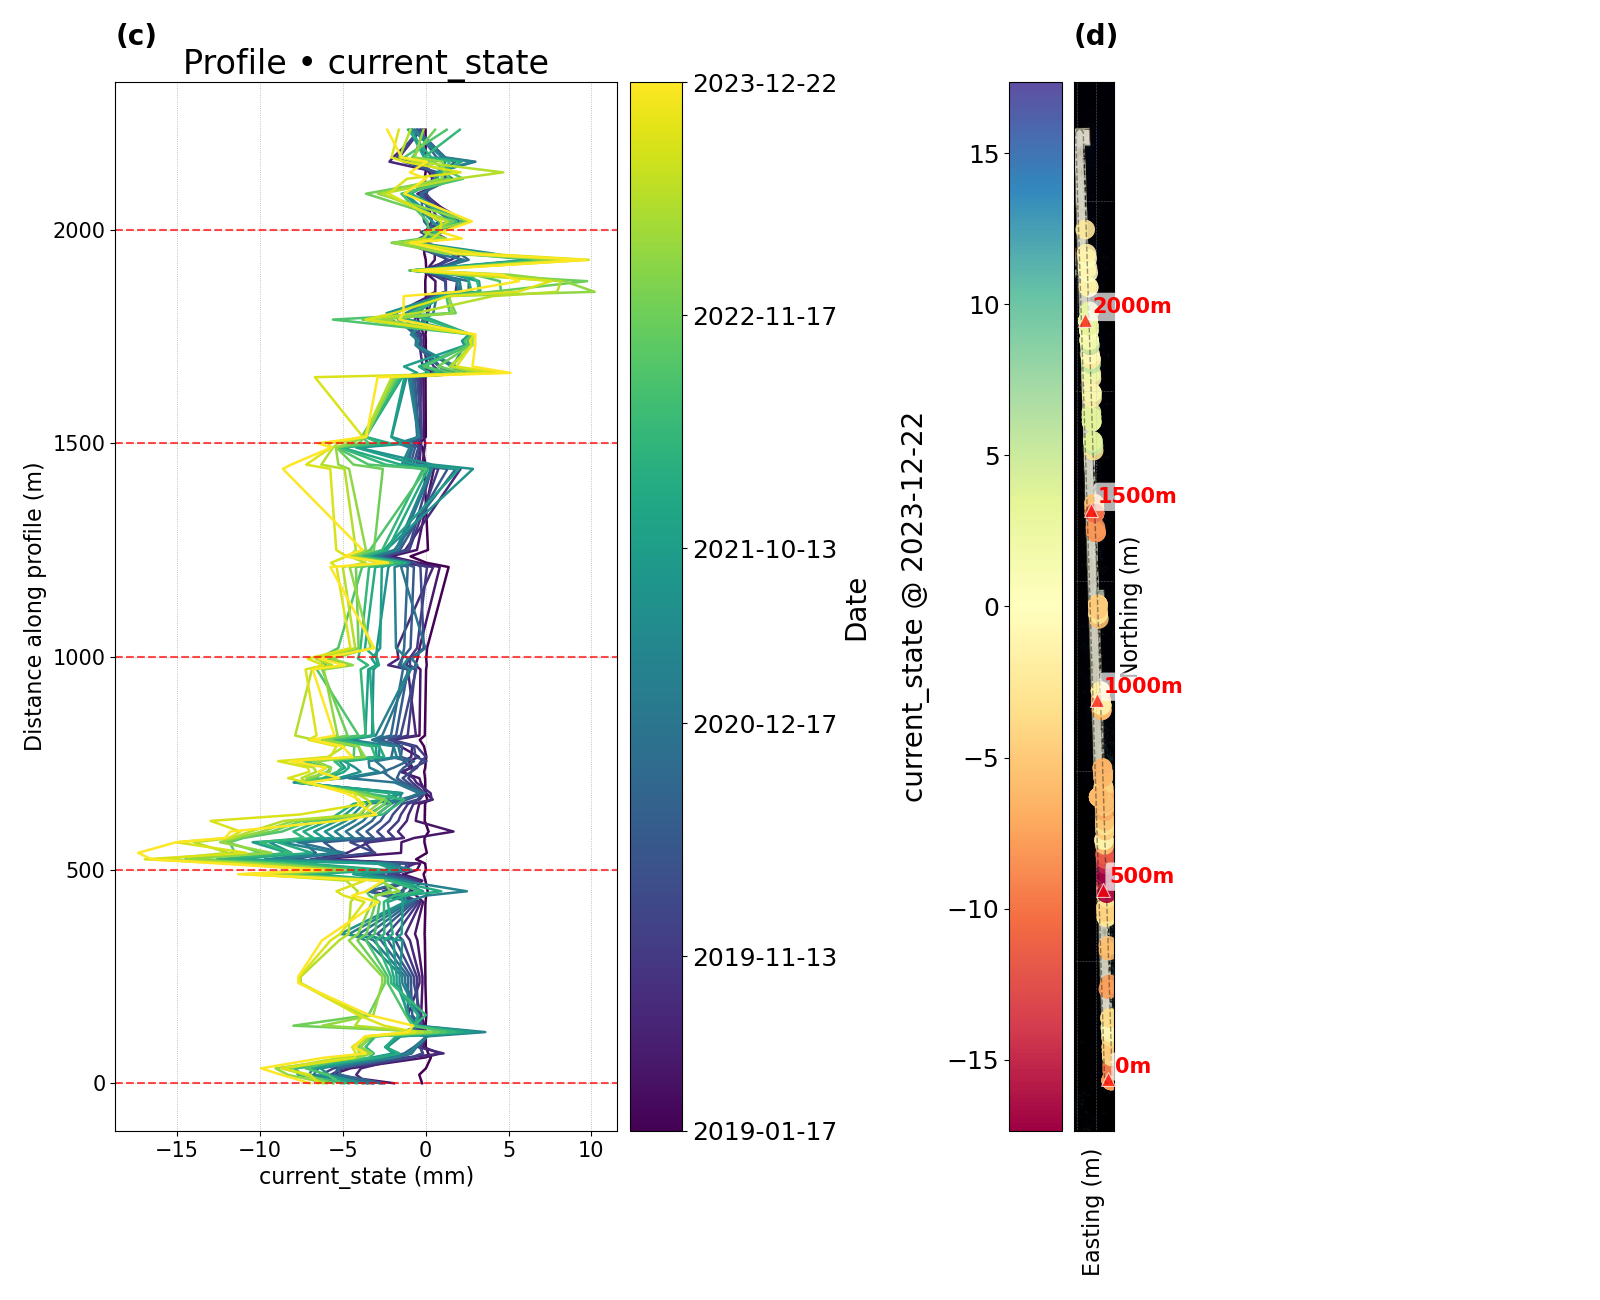
\includegraphics[width=\linewidth]{figures/ch4_algeciras_exento_profile_2.png}
  \end{columns}
\end{frame}

\begin{frame}{Sintesis VAI y metricas agregadas}
  \centering
  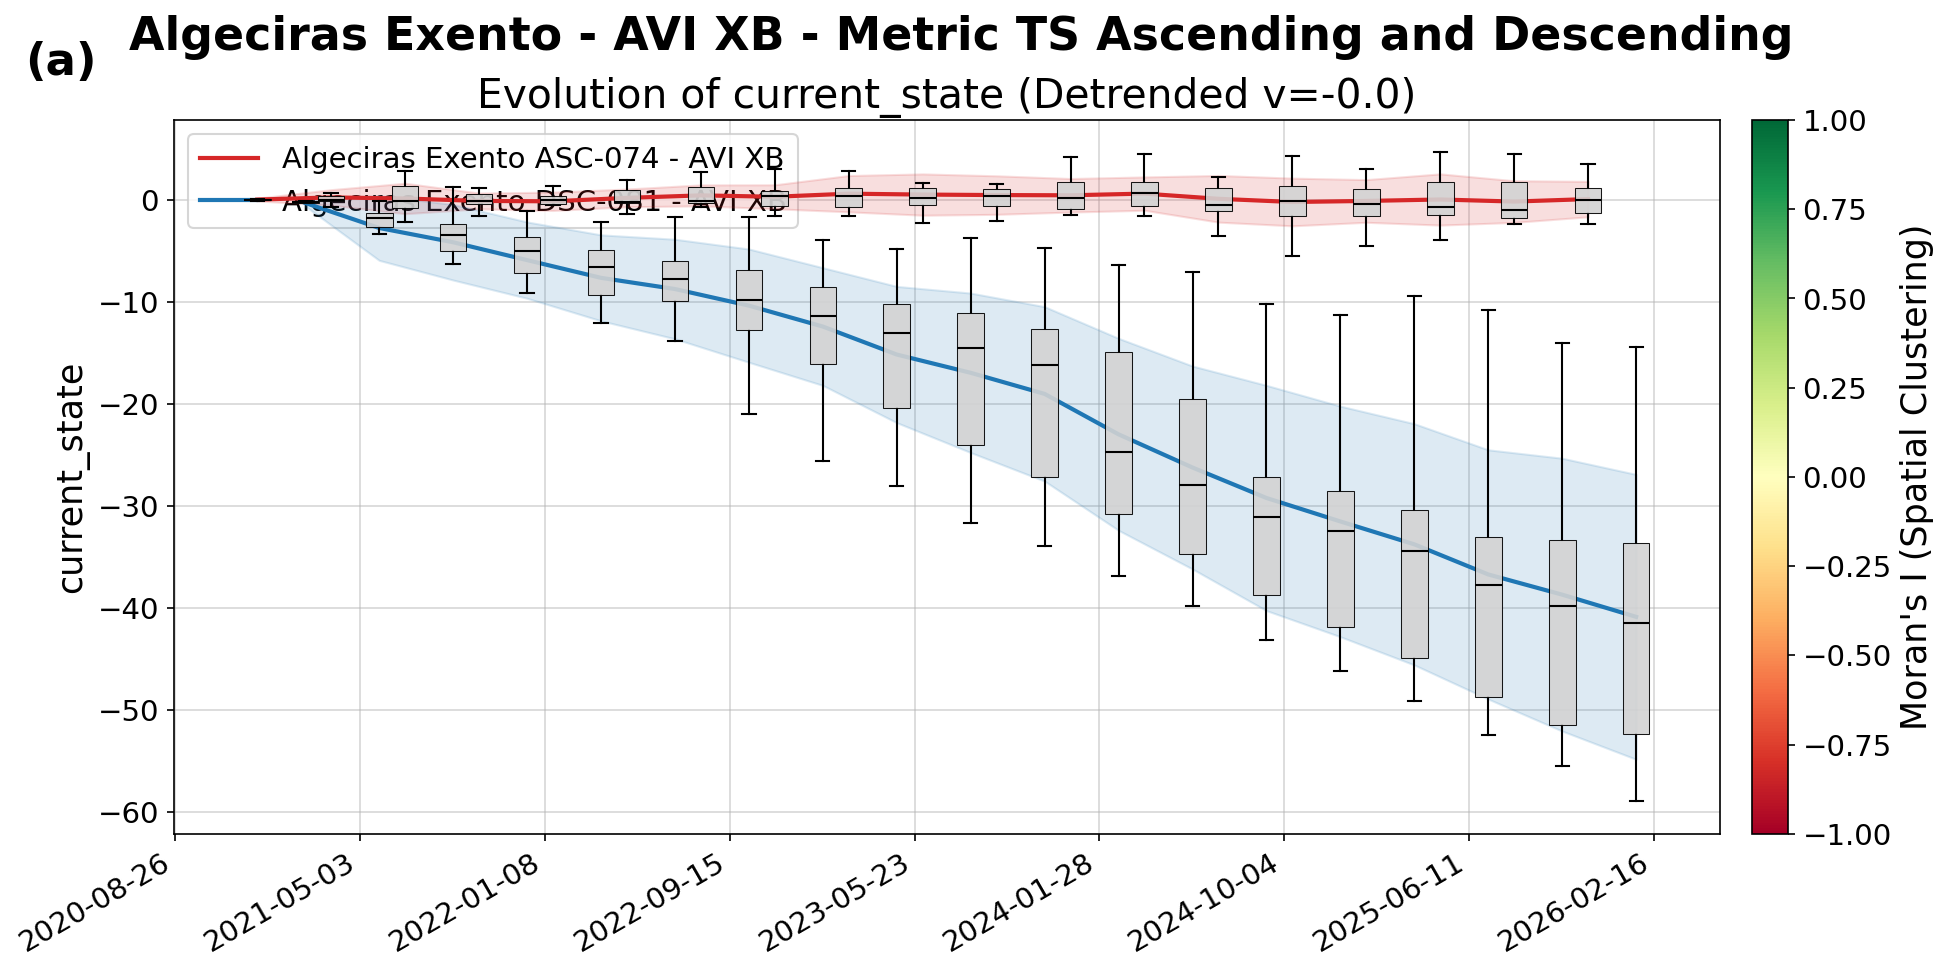
\includegraphics[width=0.78\linewidth]{figures/ch4_algeciras_xb_boxplots.png}
\end{frame}

\section{Conclusiones}

\begin{frame}{Contribuciones principales}
  \begin{itemize}
    \item Definicion del \textbf{VAI} como unidad de observacion.
    \item Flujo \textbf{CSLC + phase linking} adaptado a puertos.
    \item Atribucion \textbf{LiDAR-InSAR} con incertidumbre explicita.
    \item Interpretacion temporal con \textbf{MHT} y metricas agregadas.
    \item Conexion con el vector de riesgo $R = [P, V, C]$.
  \end{itemize}
\end{frame}

\begin{frame}{Puente entre observacion y gestion}
  \begin{itemize}
    \item La tesis convierte archivos satelitales en un observatorio comparable.
    \item El producto final ayuda a priorizar inspeccion y seguimiento.
    \item Tambien deja una base para digital twin, CMMS y alerta temprana.
  \end{itemize}
\end{frame}

\begin{frame}{Limitaciones y trabajo futuro}
  \begin{itemize}
    \item La causalidad no se infiere automaticamente: hace falta contexto e inspeccion.
    \item La geometria \texttt{C-band} limita algunos activos complejos.
    \item Futuro: \texttt{X-band}, \texttt{L-band}, estados limite y umbrales adaptativos.
  \end{itemize}
\end{frame}

\begin{frame}{Cierre}
  \begin{quote}
    Esta tesis transforma mediciones satelitales de deformacion en evidencia comparable, atribuible y util para la priorizacion del riesgo y del mantenimiento en infraestructuras portuarias.
  \end{quote}
\end{frame}

\setbeamertemplate{frame numbering}[none]
{\setbeamercolor{palette primary}{fg=white,bg=orange}
\begin{frame}[standout]
  Muchas gracias\\Preguntas
\end{frame}}

\end{document}
